\mfpicnumber{1}

\opengraphsfile{RealZeros}

\setcounter{footnote}{0}

\label{RealZeros}

In Section \ref{Polydivision}, we found that we can use synthetic division to determine if a given real number is a zero of a polynomial function.  This section presents results which will help us determine good candidates to test using synthetic division.  There are two approaches to the topic of finding the real zeros of a polynomial.  The first approach  is to use a little bit of Mathematics followed by a good use of technology like graphing utilities.  The second approach  makes good use of mathematical machinery (theorems) only.  For completeness, we include the two approaches but in separate subsections. Both approaches benefit from the following two theorems, the first of which is due to the famous mathematician \href{http://en.wikipedia.org/wiki/Cauchy}{\underline{Augustin Cauchy}}.  It gives us an interval on which \textit{all} of the real zeros of a polynomial can be found.

\smallskip

\colorbox{ResultColor}{\bbm

\begin{thm} \label{CauchysBound}\index{Cauchy's Bound}\textbf{Cauchy's Bound:}  Suppose $f(x) = a_{n} x^{n} + a_{n-\mbox{\tiny$1$}}x^{n-\mbox{\tiny$1$}} + \ldots + a_{\mbox{\tiny$1$}} x + a_{\mbox{\tiny$0$}}$ is a polynomial of degree $n$ with $n \geq 1$.  Let $M$ be the largest of the numbers: $\frac{|a_{0}|}{|a_{n}|}$, $\frac{|a_{1}|}{|a_{n}|}$, \ldots, $\frac{|a_{n-1}|}{|a_{n}|}$.  Then all the real zeros of $f$ lie in in the interval $[-(M+1),M+1]$.
\end{thm}

\ebm}


There's a lot going on in the statement of Cauchy's Bound, so we'll get right to an example and show how it is used. For those wanting a proof of Cauchy's Bound, see Exercise \ref{CauchyBoundProofExercise} in Section \ref{Summation}.


\begin{ex} \label{CBex} Let $f(x) = 2x^4+4x^3-x^2-6x-3$.  Determine an interval which contains all of the real zeros of $f$.

\smallskip

{\bf Solution.} To find the $M$ stated in Cauchy's Bound, we take the absolute value of the leading coefficient, in this case $|2| = 2$ and divide it into the largest (in absolute value) of the remaining coefficients, in this case $|-6| = 6$.   This yields $M=3$ so it is guaranteed that all of the real zeros of $f$ lie in the interval $[-4,4]$.  \qed

\end{ex}

Whereas the previous result tells us \textit{where} we can find the real zeros of a polynomial, the next theorem gives us a list of \textit{possible} real zeros.

\smallskip

\colorbox{ResultColor}{\bbm

\begin{thm} \label{RZT}\index{Rational Zeros Theorem}\textbf{Rational Zeros Theorem:}  Suppose $f(x) = a_{n} x^{n} + a_{n-\mbox{\tiny$1$}}x^{n-\mbox{\tiny$1$}} + \ldots + a_{\mbox{\tiny$1$}} x + a_{\mbox{\tiny$0$}}$ is a polynomial of degree $n$ with $n \geq 1$, and $a_{\mbox{\tiny$0$}}$, $a_{\mbox{\tiny$1$}}$, \ldots $a_{n}$ are integers.  If $r$ is a rational zero of $f$, then $r$ is of the form $\pm \frac{p}{q}$, where $p$ is a factor of the constant term $a_{\mbox{\tiny$0$}}$, and $q$ is a factor of the leading coefficient $a_{n}$.  
\end{thm}

\ebm}

\smallskip

The Rational Zeros Theorem gives us a list of numbers to try in our synthetic division and that is a lot nicer than simply guessing.  If none of the numbers in the list are zeros, then either the polynomial has no real zeros at all, or all of the real zeros are irrational numbers.  To see why the Rational Zeros Theorem works, suppose $c$ is a zero of $f$ and $c = \frac{p}{q}$ in lowest terms.  This means $p$ and $q$ have no common factors.  Since $f(c) = 0$, we have \[a_{n} \left(\frac{p}{q}\right)^{n} + a_{n-\mbox{\tiny$1$}}\left(\frac{p}{q}\right)^{n-\mbox{\tiny$1$}} + \ldots + a_{\mbox{\tiny$1$}} \left(\frac{p}{q}\right) + a_{\mbox{\tiny$0$}} = 0.\]  Multiplying both sides of this equation by $q^n$, we clear the denominators to get \[a_{n}p^{n} + a_{n-\mbox{\tiny$1$}}p^{n-\mbox{\tiny$1$}}q + \ldots + a_{\mbox{\tiny$1$}}p q^{n-\mbox{\tiny$1$}} + a_{\mbox{\tiny$0$}}q^n = 0\]  Rearranging this equation, we get  \[a_{n}p^{n} = -a_{n-\mbox{\tiny$1$}}p^{n-\mbox{\tiny$1$}}q - \ldots - a_{\mbox{\tiny$1$}}p q^{n-\mbox{\tiny$1$}} -a_{\mbox{\tiny$0$}}q^n\] Now, the left hand side is an integer multiple of $p$, and the right hand side is an integer multiple of $q$. (Can you see why?)  This means $a_{n}p^{n}$ is both a multiple of $p$ and a multiple of $q$.  Since $p$ and $q$ have no common factors, $a_{n}$ must be a multiple of $q$.  If we rearrange the equation \[a_{n}p^{n} + a_{n-\mbox{\tiny$1$}}p^{n-\mbox{\tiny$1$}}q + \ldots + a_{\mbox{\tiny$1$}}p q^{n-\mbox{\tiny$1$}} + a_{\mbox{\tiny$0$}}q^n = 0\] as \[a_{\mbox{\tiny$0$}}q^n = -a_{n}p^{n} - a_{n-\mbox{\tiny$1$}}p^{n-\mbox{\tiny$1$}}q - \ldots - a_{\mbox{\tiny$1$}}p q^{n-\mbox{\tiny$1$}}\] we can play the same game and conclude $a_{\mbox{\tiny$0$}}$ is a multiple of $p$, and we have the result.

\begin{ex}  Let $f(x) = 2x^4+4x^3-x^2-6x-3$. Use the Rational Zeros Theorem to list all of the possible rational zeros of $f$.

\smallskip

{\bf Solution.}  To generate a complete list of rational zeros, we need to take each of the factors of constant term, $a_{\mbox{\tiny$0$}} = -3$, and divide them by each of the factors of the leading coefficient $a_{\mbox{\tiny$4$}} = 2$.  The factors of $-3$ are $\pm \, 1$ and $\pm \, 3$.  Since the Rational Zeros Theorem tacks on a $\pm$ anyway, for the moment, we consider only the positive factors $1$ and $3$.  The factors of $2$ are  $1$ and $2$, so the Rational Zeros Theorem gives the list $\left\{\pm \, \frac{1}{1}, \pm \, \frac{1}{2},  \pm \, \frac{3}{1}, \pm \, \frac{3}{2}\right\}$ or $\left\{\pm \, \frac{1}{2}, \pm \, 1, \pm \, \frac{3}{2}, \pm \, 3\right\}$. \qed
\label{RZTex}
\end{ex}

Our discussion now diverges between those who wish to use technology and those who do not.  

\subsection{For Those Wishing to use a Graphing Utility}

At this stage, we know not only the interval in which all of the zeros of $f(x) = 2x^4+4x^3-x^2-6x-3$ are located, but we also know some potential candidates.  We can now use our calculator to help us determine all of the real zeros of $f$, as illustrated in the next example.

\begin{ex}  Let $f(x) = 2x^4+4x^3-x^2-6x-3$.  

\begin{enumerate}

\item  Graph $y=f(x)$ using a graphing utility over the interval  obtained in Example \ref{CBex}.

\item  Use the graph to shorten the list of possible rational zeros obtained in Example \ref{RZTex}.

\item  Use synthetic division to find the real zeros of $f$, and state their multiplicities.


\end{enumerate}

{\bf Solution.}

\begin{enumerate}

\item  In Example \ref{CBex}, we determined all of the real zeros of $f$ lie in the interval $[-4, 4]$, so we restrict our attention to that portion of the $x$-axis.

\item  In Example \ref{RZTex}, we learned that any rational zero of $f$ must be in the list $\left\{\pm \, \frac{1}{2}, \pm \, 1, \pm \, \frac{3}{2}, \pm \, 3\right\}$.  From the graph, it looks as if we can rule out any of the positive rational zeros, since the graph seems to cross the $x$-axis at $x \approx 1.225$.  On the negative side, $x=-1$ looks good. Indeed,  the shape  of the graph near $(-1,0)$ suggests that if $x=-1$ is a zero, it is of multiplicity at least three.  We set about synthetically dividing:
 
\[\begin{array}{rrrrrr}

 -1 \, \, \vline& 2 & 4 & -1  & -6 & -3 \\

  & \downarrow     &  -2  &  -2  & 3 & 3\\ \hhline{~-----} 
  
  &  2            &   2  & -3 & -3 &  \fbox{$0$}  \\

\end{array}\]

Since $f$ is a fourth degree polynomial, we know that our quotient is a third degree polynomial.  If we can do one more successful division, we will have reduced the quotient  to a quadratic, and we can use the quadratic formula, if needed, to find the two  remaining  zeros.  Continuing with $x=-1$:

\[\begin{array}{rrrrrr}
 -1 \, \, \vline& 2 & 4 & -1  & -6 & -3 \\

  & \downarrow     &  -2  &  -2  & 3 & 3\\ \hhline{~-----} 
  
  -1 \, \, \vline&  2 &   2  & -3 & -3 &  \fbox{$0$}  \\
    
               & \downarrow &  -2  &  0  & 3 &\\ \hhline{~----} 
 
   & 2  &   0  & -3& \fbox{0} &   \\
  
        

\end{array}\]

 Our quotient polynomial is now $2x^2 - 3$.  Setting this to zero gives $2x^2 - 3 = 0$, or $x^2 = \frac{3}{2}$, which gives us $x = \pm \, \frac{\sqrt{6}}{2}$.  Based on our division work, we know that $-1$ has a multiplicity of \textit{at least} $2$. The Factor Theorem tells us our remaining zeros, $\pm \, \frac{\sqrt{6}}{2}$, each have multiplicity at least $1$.  However, Theorem \ref{nzerosreal} tells us $f$ can have at most $4$ real zeros, counting multiplicity, and so we conclude that $-1$ is of multiplicity \textit{exactly} $2$ and $\pm \, \frac{\sqrt{6}}{2} \approx \pm 1.225$ each has multiplicity $1$. Thus, we were incorrect in thinking  $-1$ was a zero of multiplicity $3$.  Sure enough, if we adjust zoom in near $(-1,0)$ using graphing utility, we find the graph of $y = f(x)$ touches and rebounds from the $x$-axis at $(-1,0)$, typical behavior near a zero of even multiplicity. The lesson here is, once again, technology may \textit{suggest} a result, but it is only the mathematics which can \textit{prove} (or in this case, \textit{disprove}) it.  

\end{enumerate}

\begin{center}

\begin{tabular}{cc}

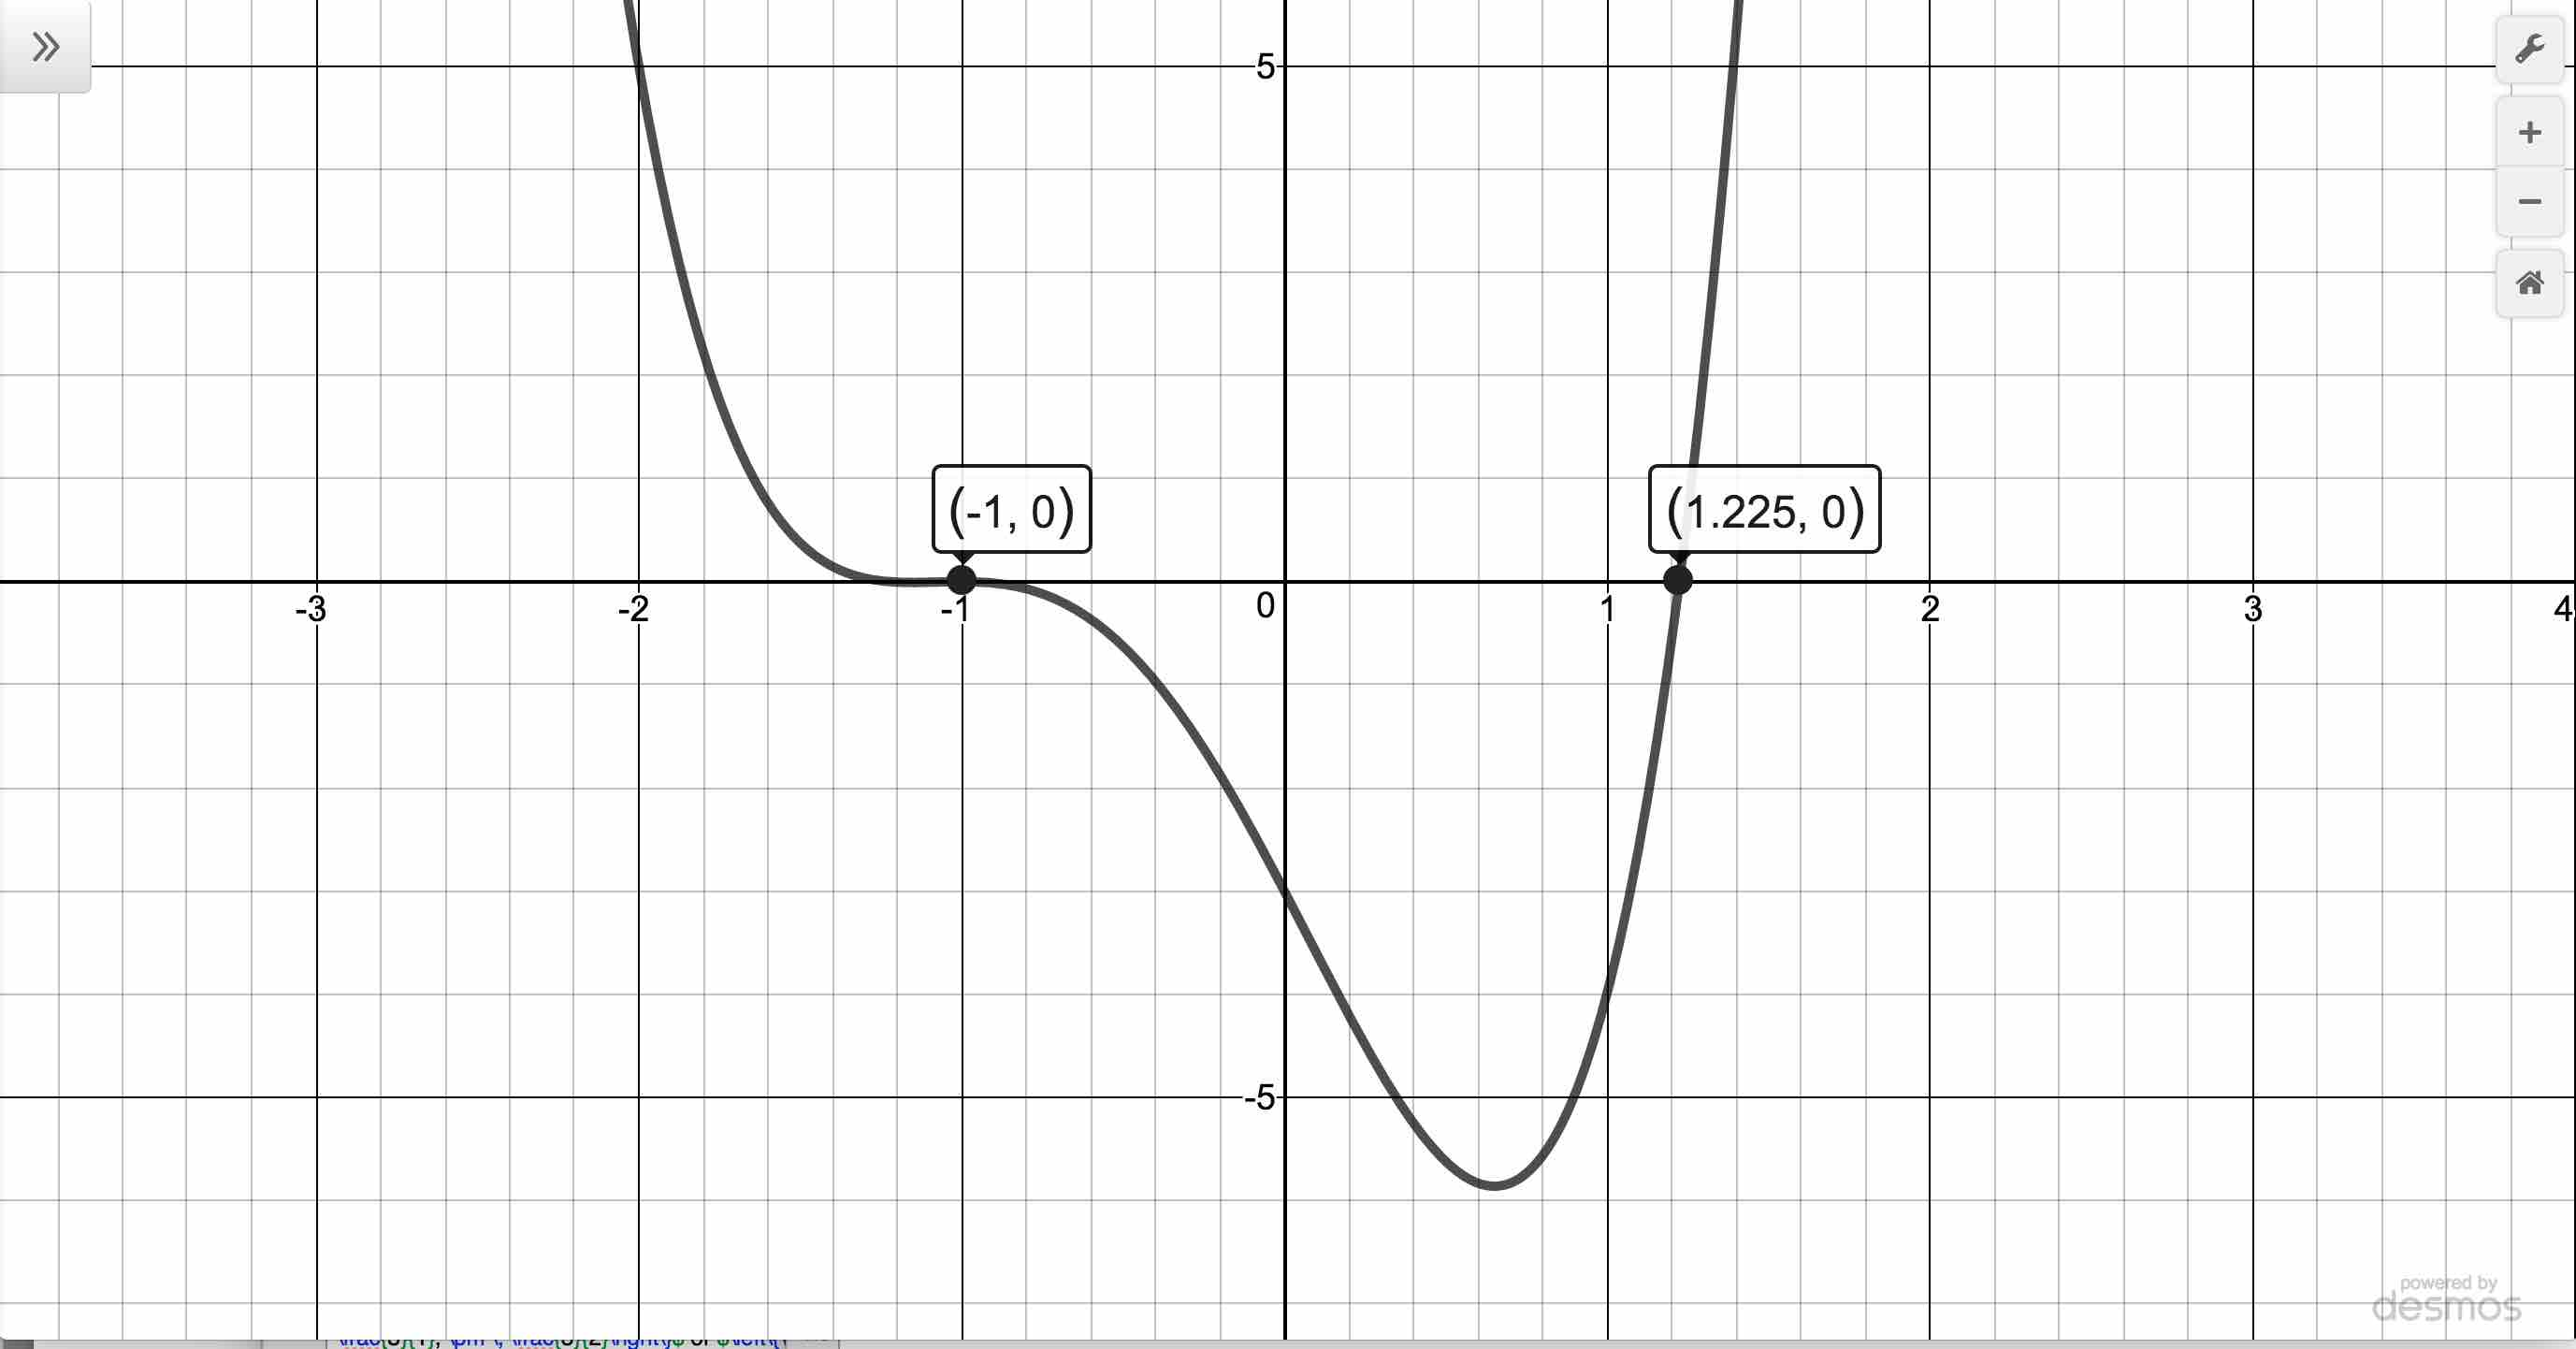
\includegraphics[width = 3in, height=2in]{./RealZerosGraphics/RealZerosEx01a.jpg}  &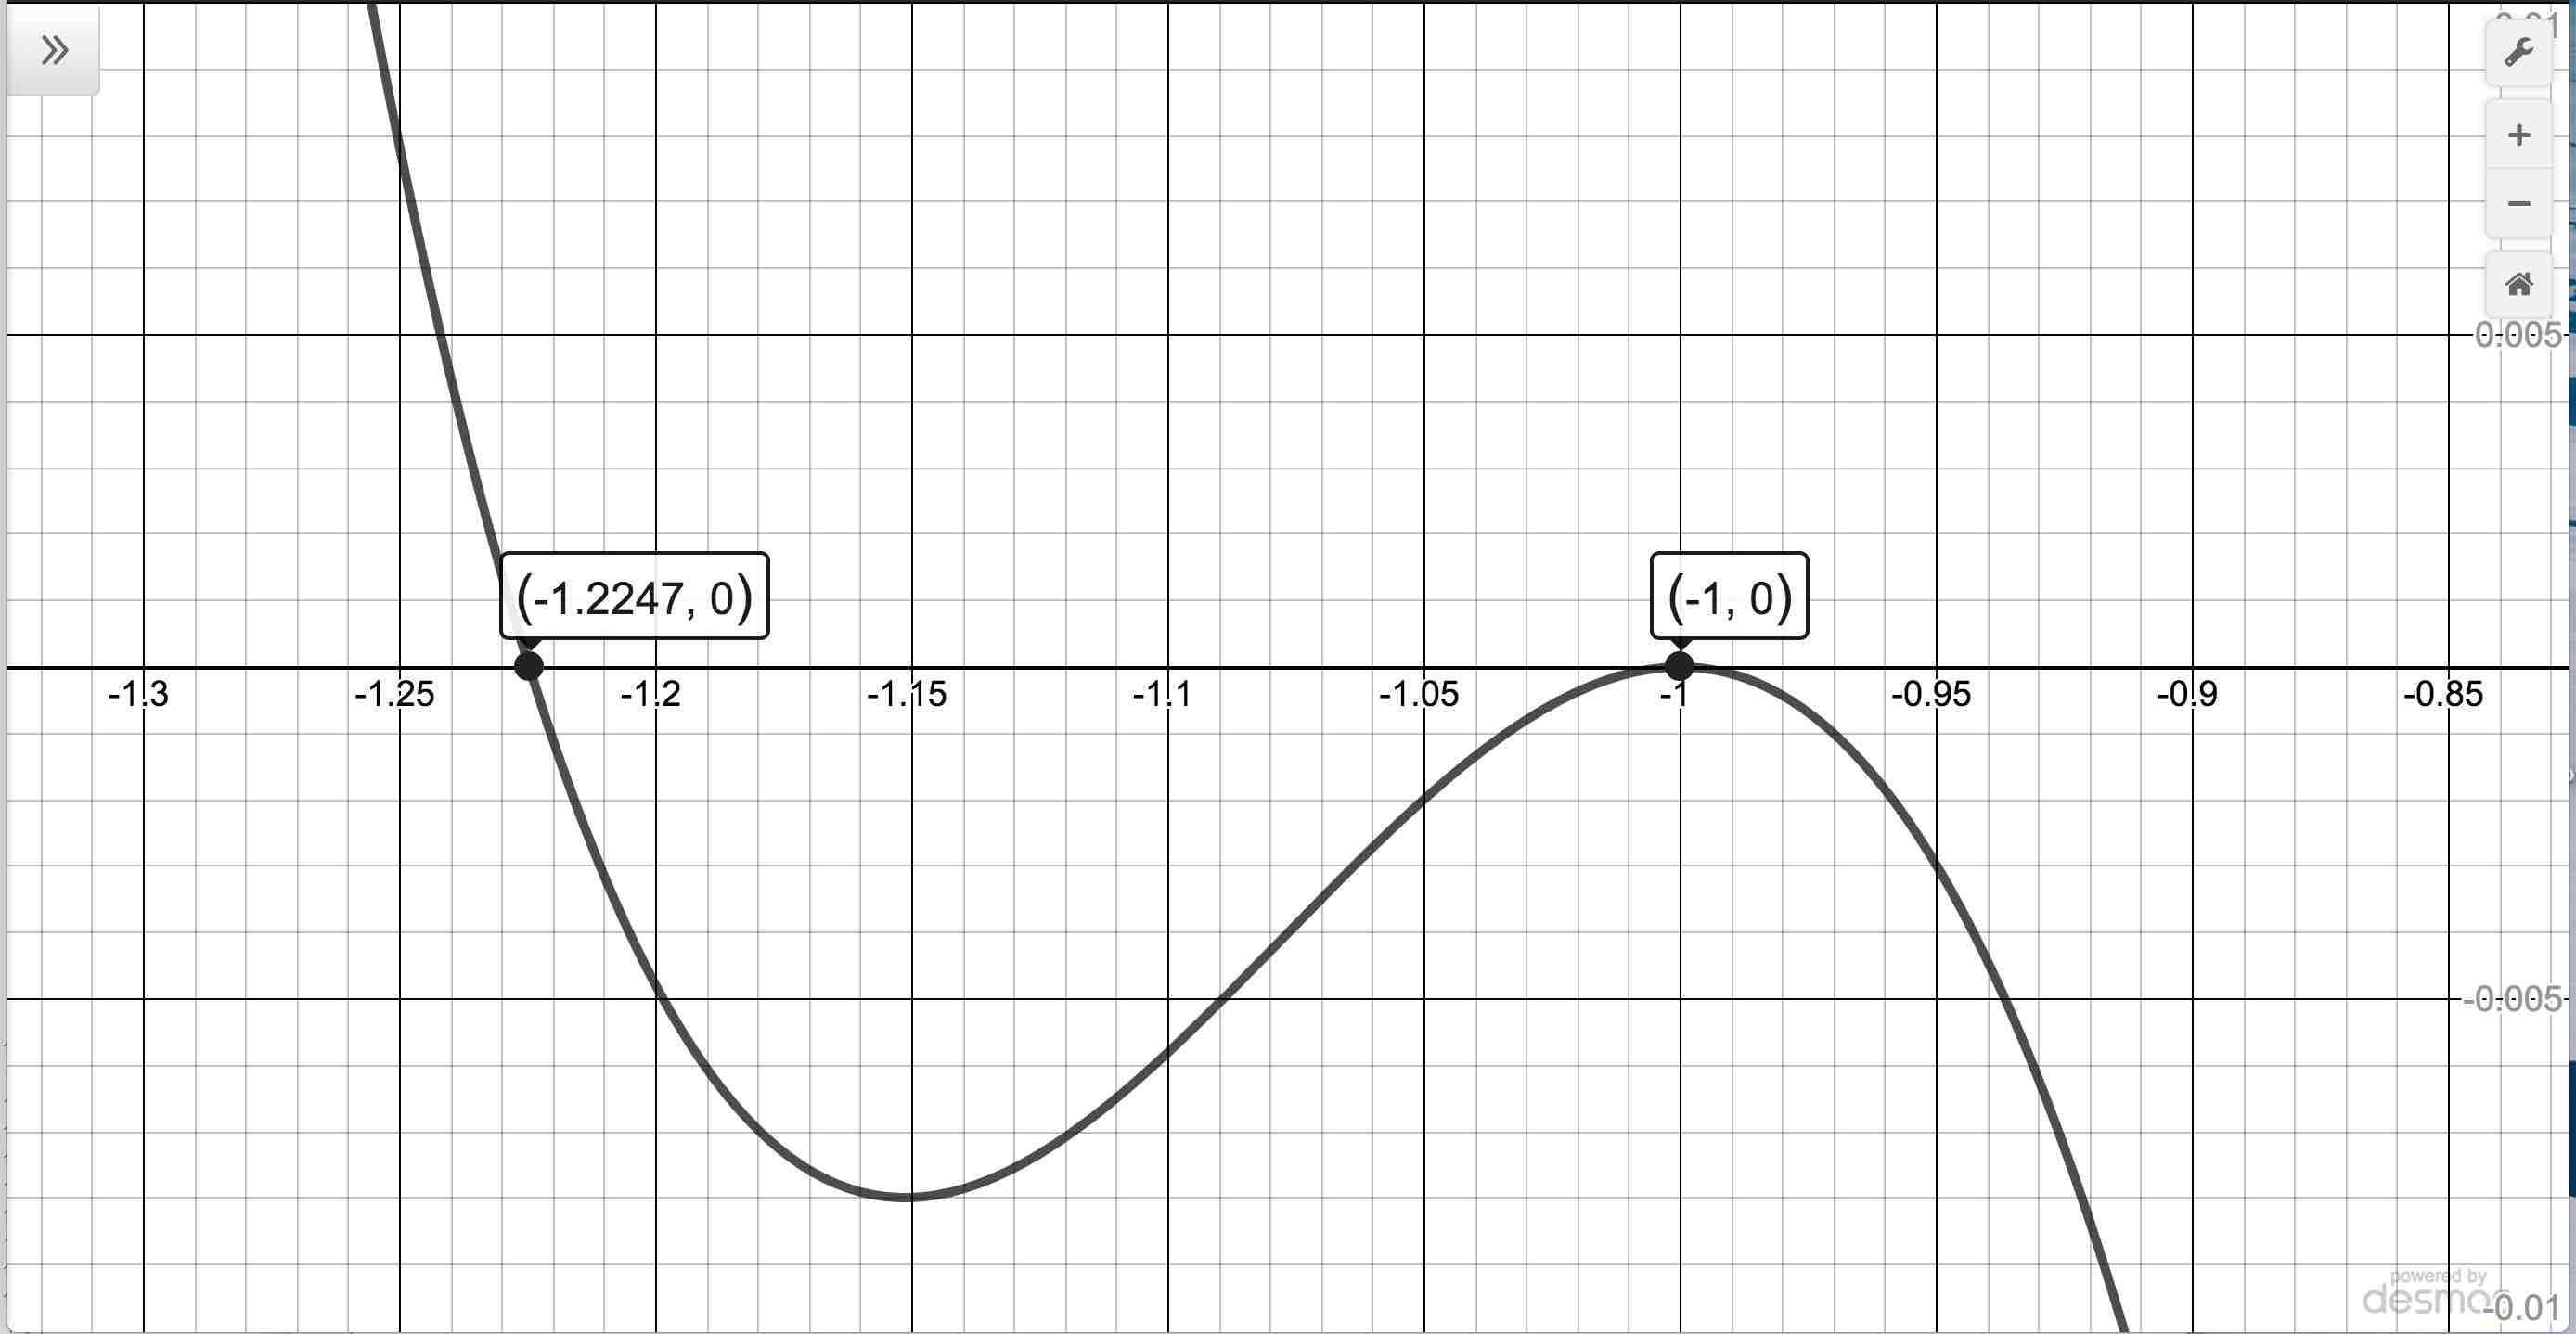
\includegraphics[width = 3in, height=2in]{./RealZerosGraphics/RealZerosEx01b.jpg}

\end{tabular}
\end{center}

 \qed

\end{ex}


Our next example shows how even a mild-mannered polynomial can cause problems.

\begin{ex}  \label{polyquadinform} Let $f(x) = x^4 + x^2 - 12$.

\begin{enumerate}

\item  Use Cauchy's Bound to determine an interval in which all of the real zeros of $f$ lie.

\item  Use the Rational Zeros Theorem to determine a list of possible rational zeros of $f$.

\item  Graph $y=f(x)$ using a graphing utility.

\item  Find all of the real zeros of $f$ and their multiplicities.


\end{enumerate}

{\bf Solution.}

\begin{enumerate}

\item  Applying Cauchy's Bound, we find $M = 12$, so all of the real zeros lie in the interval $[-13,13]$.

\item  Applying the Rational Zeros Theorem with constant term $a_{\mbox{\tiny$0$}} = -12$ and leading coefficient $a_{\mbox{\tiny$4$}} = 1$, we get the list $\{\pm \, 1$, $\pm \, 2$, $\pm \, 3$, $\pm \, 4$, $\pm \, 6$, $\pm \, 12\}$.

\item  Graphing $y=f(x)$ on the interval $[-13,13]$ produces the graph below on the left.  Zooming in a bit gives the graph below on the right.  Based on the graph, none of our rational zeros will work. (Do you see why not?)


\begin{center}

\begin{tabular}{cc}

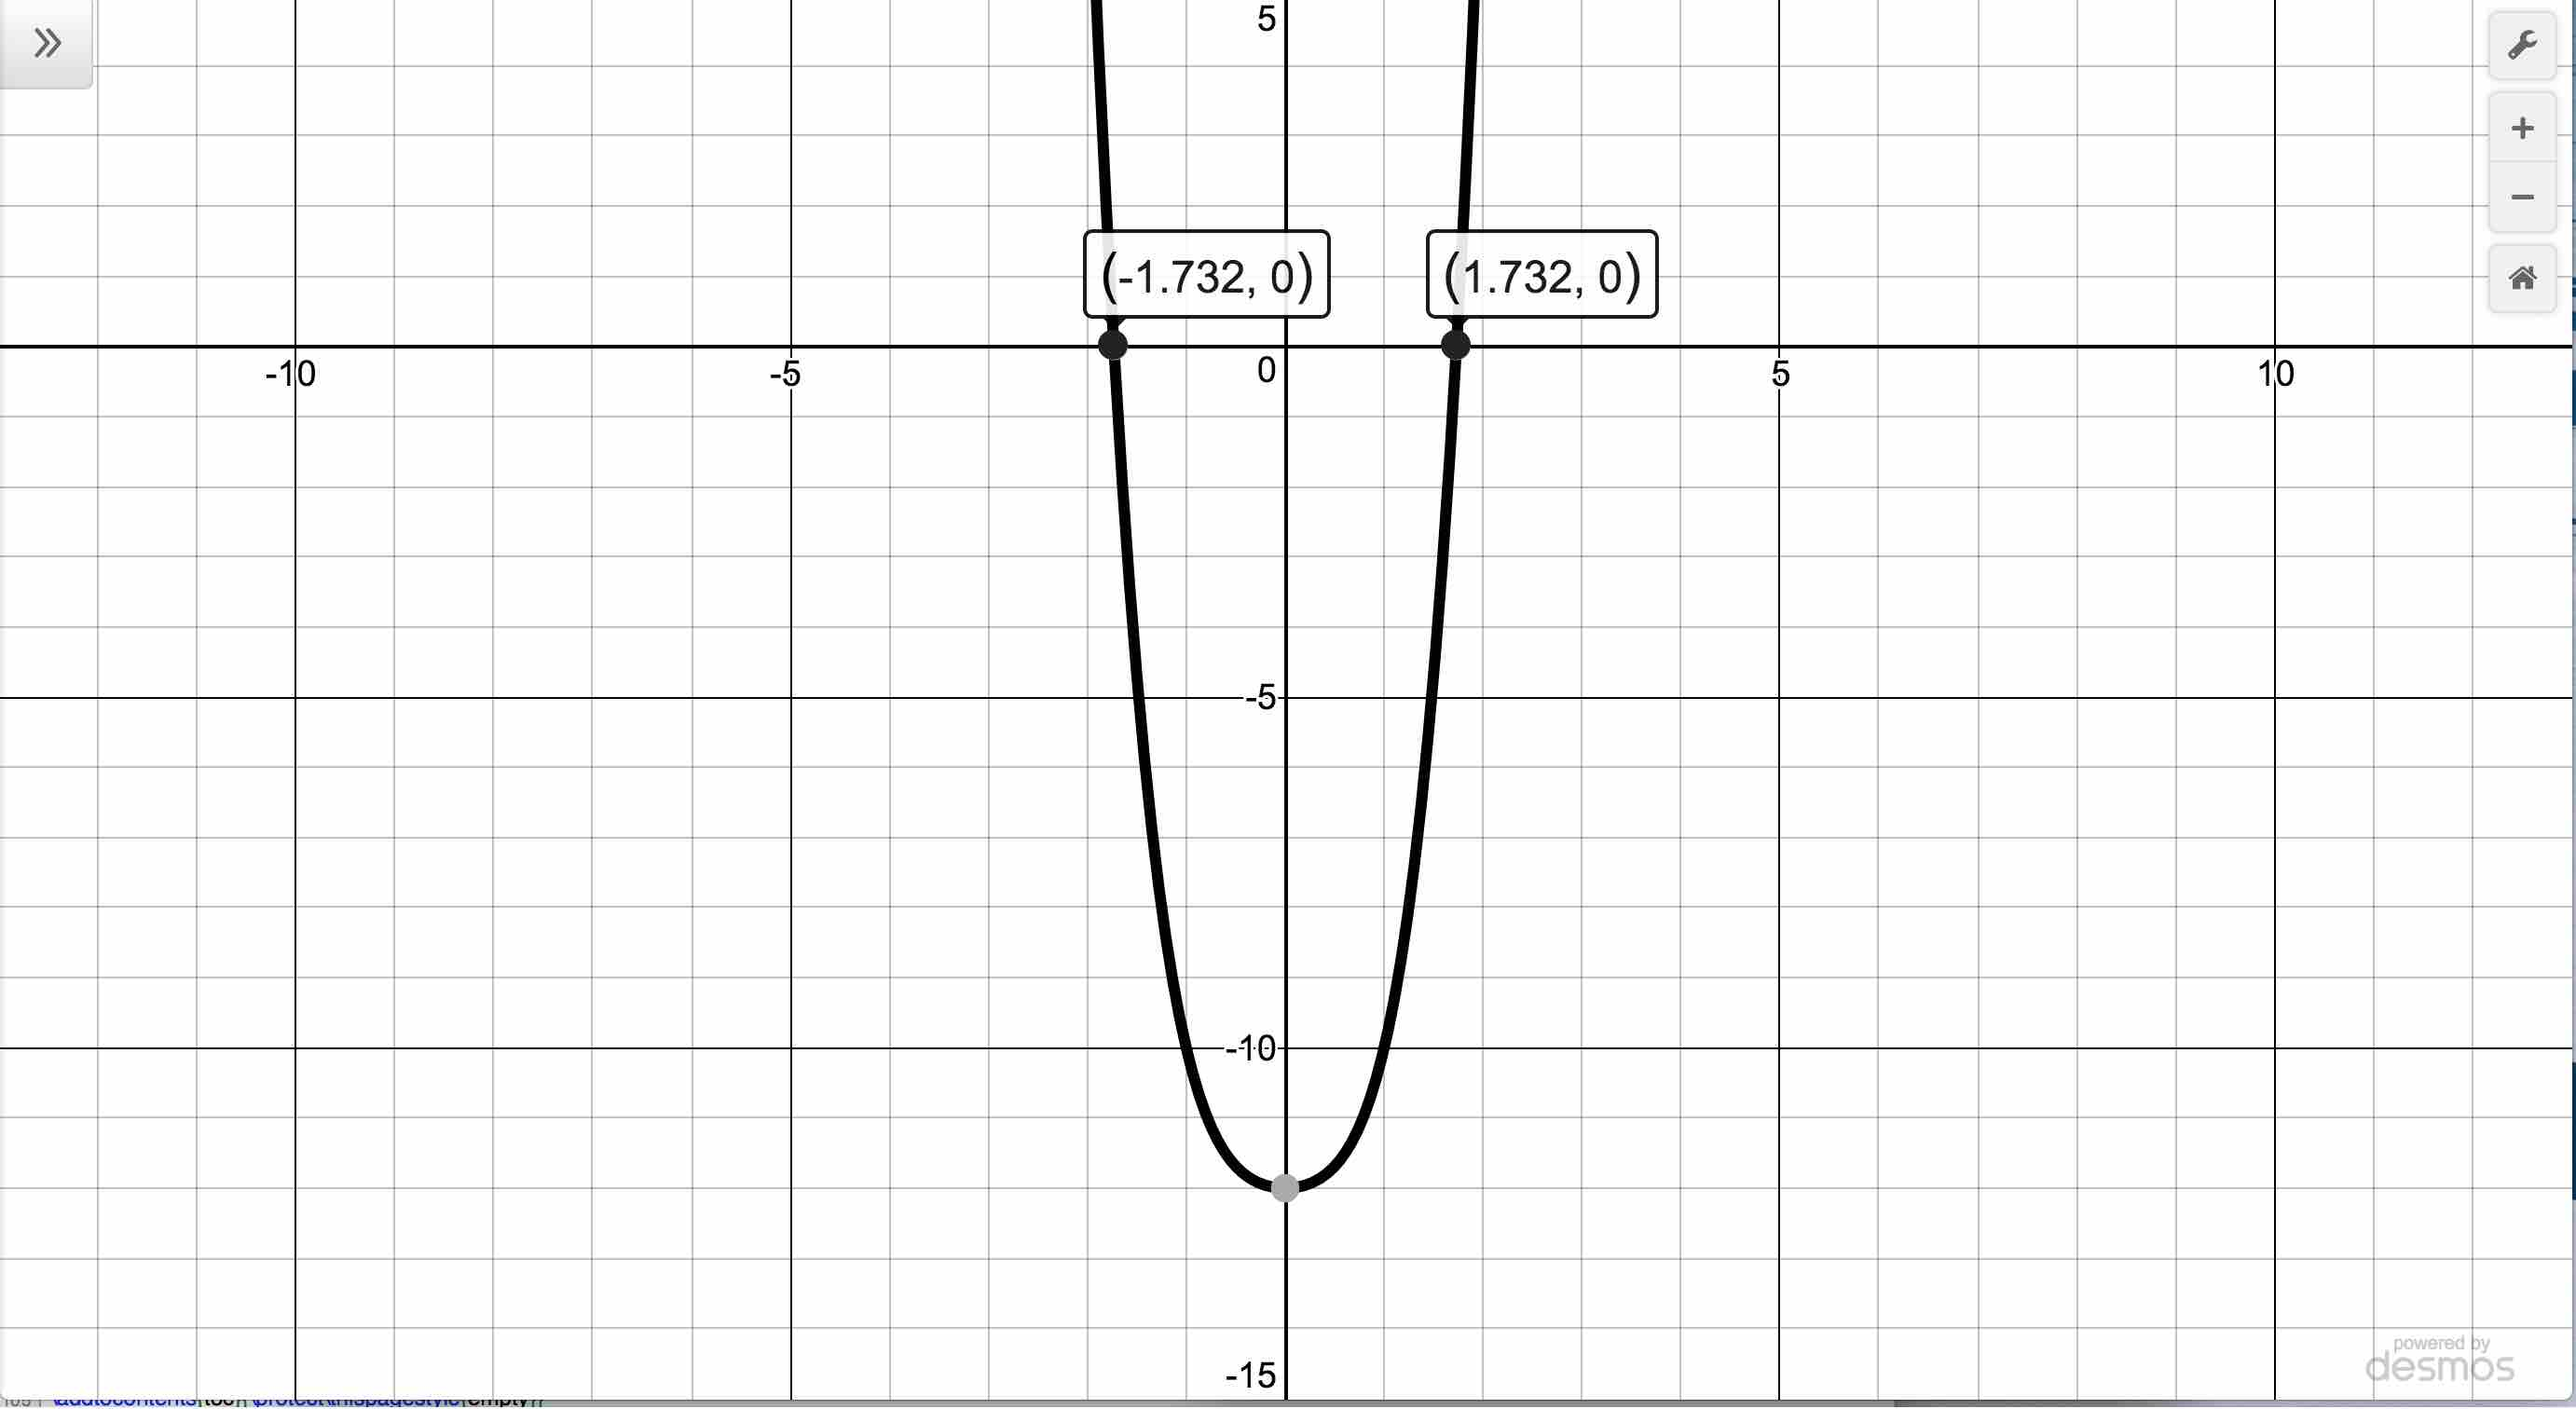
\includegraphics[width = 3in, height=2in]{./RealZerosGraphics/RealZerosEx02a.jpg}  &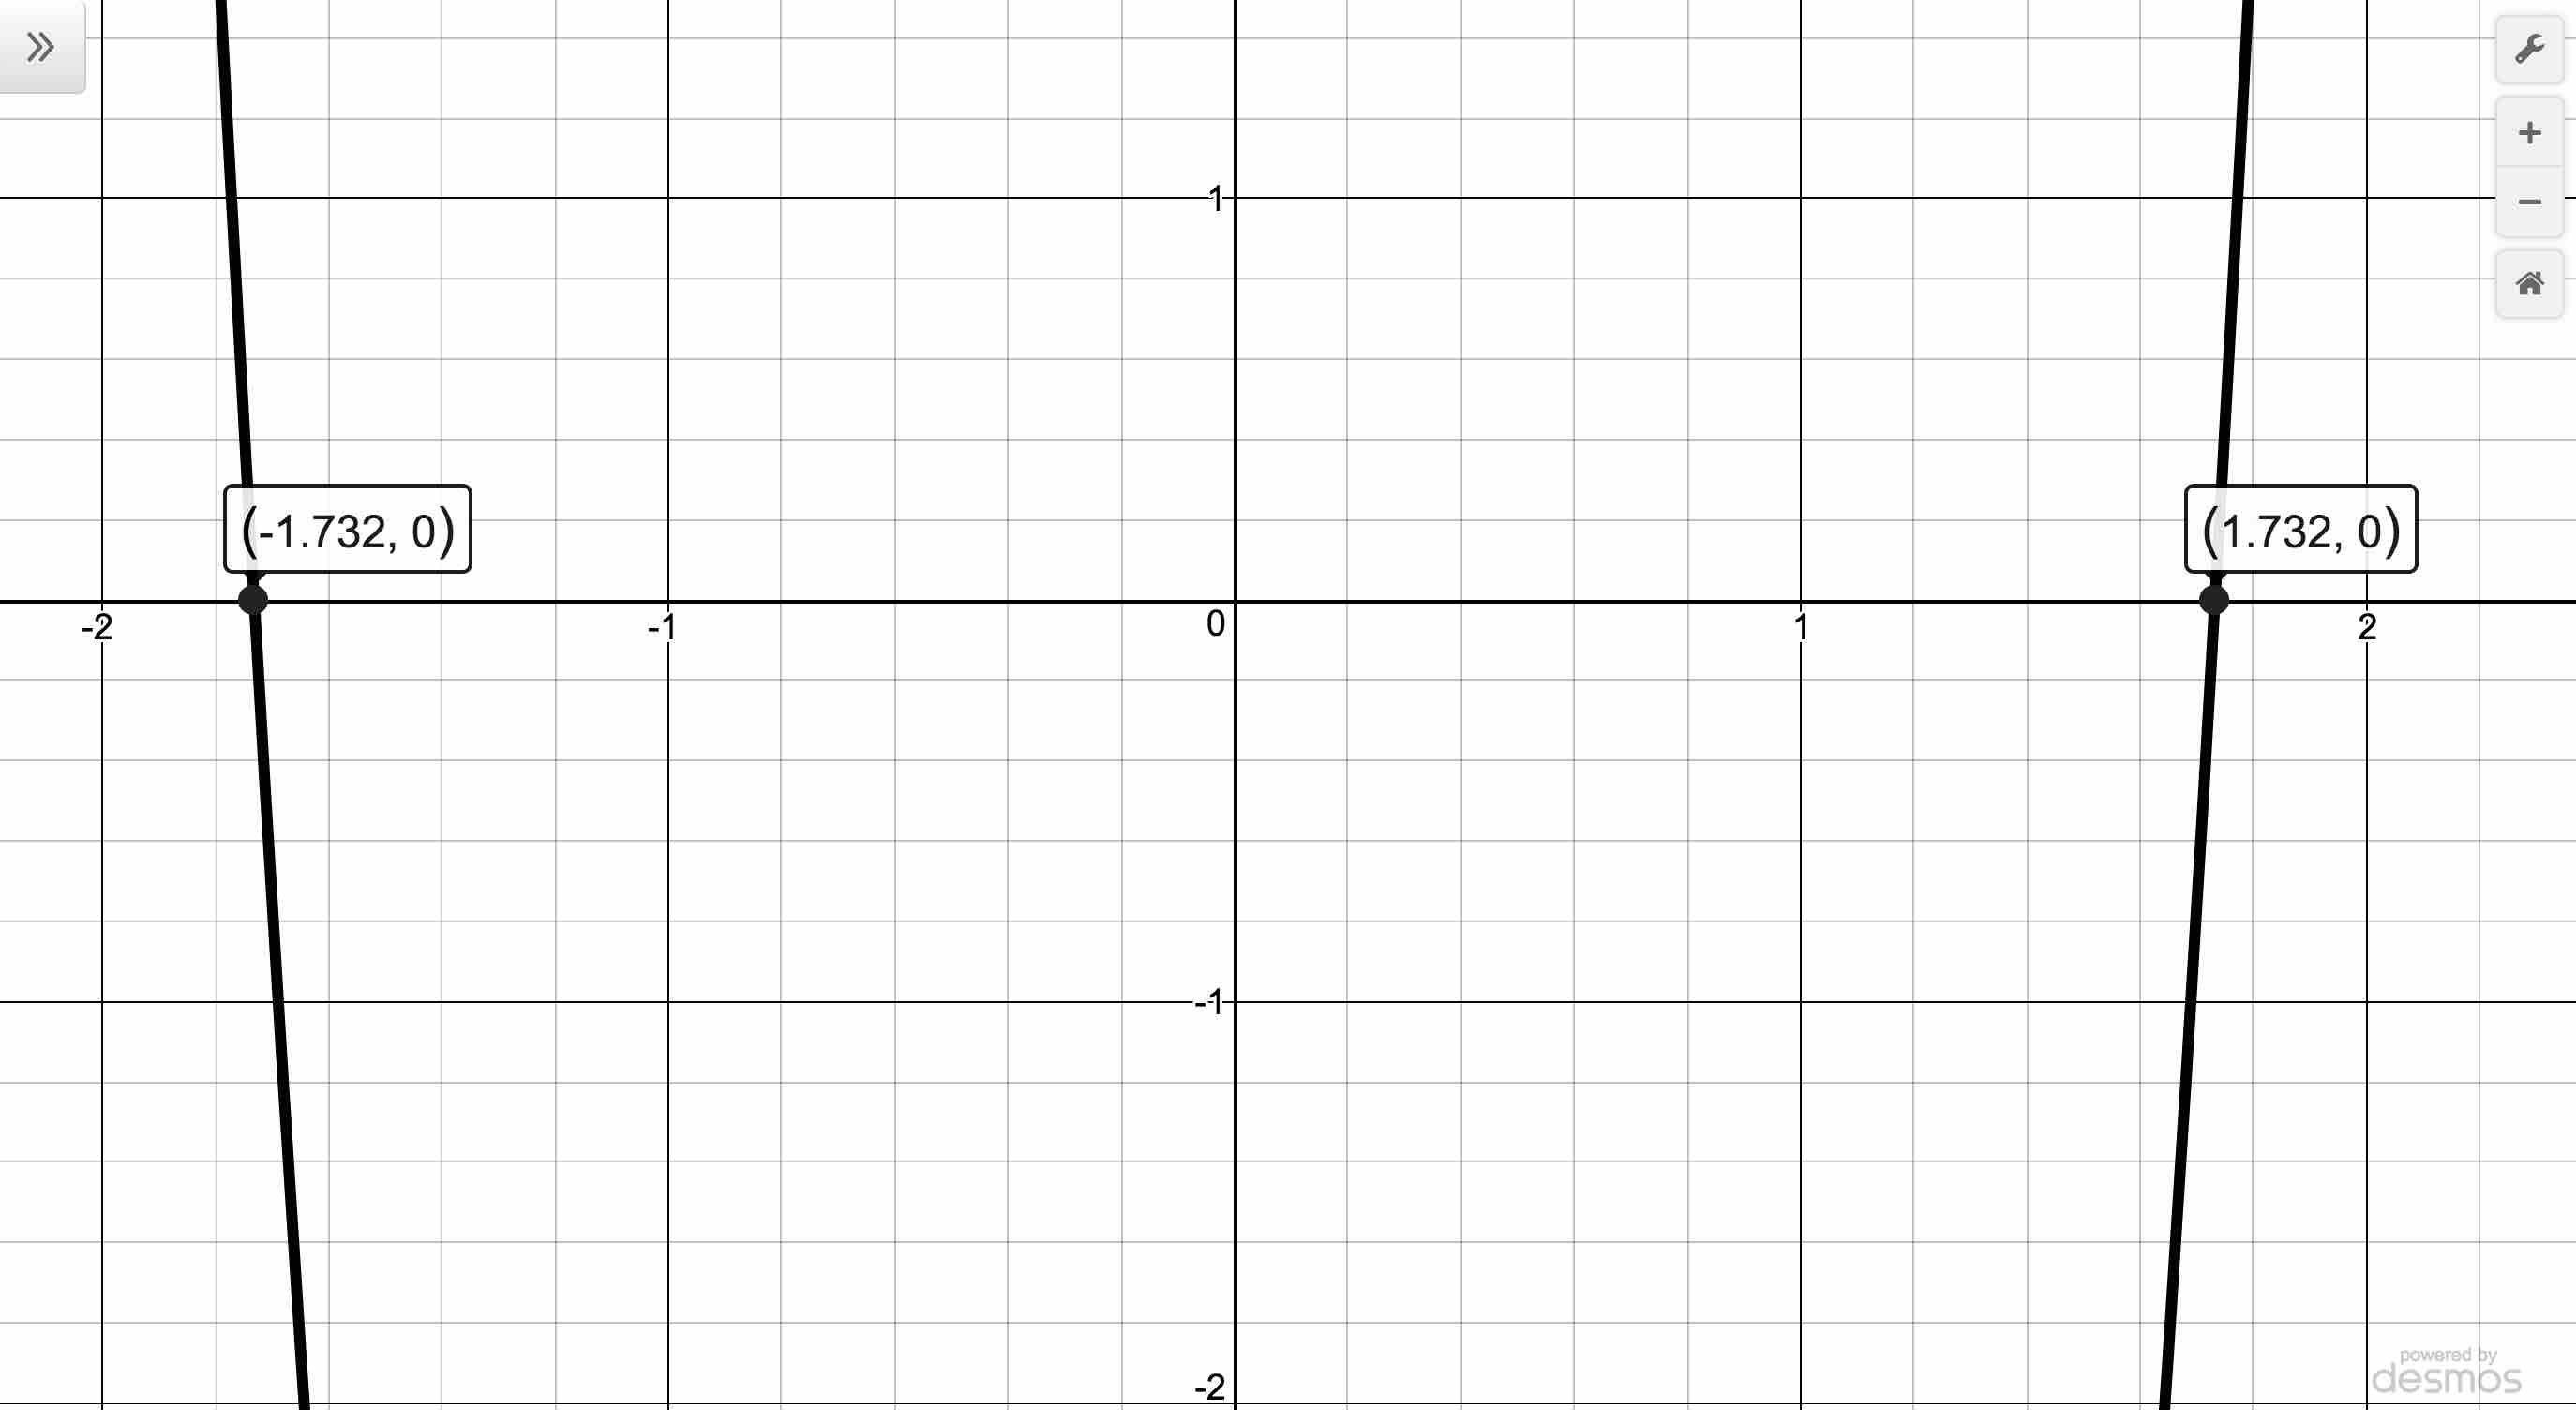
\includegraphics[width = 3in, height=2in]{./RealZerosGraphics/RealZerosEx02b.jpg}

\end{tabular}
\end{center} 

\item  From the graph, we know $f$ has two real zeros, one positive, and one negative.  Our only hope at this point is to try and find the zeros of $f$ by setting $f(x)=x^4+x^2-12=0$ and solving.  If we stare at this equation long enough, we may recognize it as a `quadratic in disguise' or `quadratic in form'. (See Section \ref{AppQuadEqus}.)   In other words, we have three terms: $x^4$, $x^2$ and $12$, and the exponent on the first term, $x^4$, is exactly twice that of the second term, $x^2$.  We may rewrite this as $\left(x^2\right)^2 + \left(x^2\right) - 12 = 0$.  To better see the forest for the trees, we momentarily replace $x^2$ with the variable $u$.  In terms of $u$, our equation becomes $u^2 + u - 12 = 0$, which we can readily factor as $(u+4)(u-3) = 0$.  In terms of $x$, this means $x^4+x^2-12= \left(x^2-3\right) \left(x^2 + 4 \right)=0$. We get $x^2 = 3$, which gives us $x = \pm \sqrt{3}$, or $x^2=-4$, which admits no real solutions.  Since $\sqrt{3} \approx 1.73$, the two zeros match what we expected from the graph.  Turning our attention now to multiplicities, the Factor Theorem guarantees that since $x = \pm \sqrt{3}$ are zeros, $(x- \sqrt{3})$ and $(x + \sqrt{3})$ are factors of $f(x)$.  We've already partially factored  $f(x)$ as $f(x)  = \left(x^2-3\right) \left(x^2 + 4 \right)$.  Since $x^2+4$ as no real zeros, we know both $(x-\sqrt{3})$ and $(x+\sqrt{3})$ must divide $x^2-3$.  By Theorem \ref{nzerosreal},  $x^2-3$ can only have a total of two zeros, including multiplicities, so we are forced to conclude $x = \pm \sqrt{3}$ are each zeros of multiplicity $1$ of $x^2-3$, and hence, $f(x)$.\footnote{Alternatively, we could recognize $x^2 -3 = x^2-(\sqrt{3})^2 = (x-\sqrt{3})(x+\sqrt{3})$, but the above argument works for all quadratic functions, even those which aren't as easy to factor.} \qed

\end{enumerate}

\label{usubex}

\end{ex}

A couple of remarks are in order.  First, the graph of $f(x) = x^4 + x^2 - 12$ appears to be symmetric about the $y$-axis.  Sure enough, we find $f(-x) = (-x)^4+(-x)^2  - 12 = x^4+x^2=12 = f(x)$ proving $f$ is, indeed, an even function, thus \textit{proving} the symmetry \textit{suggested} by the graph.  Second, the technique used to factor $f(x)$ in Example \ref{usubex} is called \index{$u$-substitution} \textbf{{\boldmath $u$}-substitution}.  We shall this technique now and then in the sections to come, so it is worth taking the time to let this idea sink in.  In general, substitution can help us identify a `quadratic in disguise' - in essence, it helps us `see the forest for the trees.'  Last, but not least, it is entirely possible that a polynomial has no real roots at all, or worse, it has real roots but none of the techniques discussed in this section can help us find them exactly.  In the latter case, we are forced to approximate using technology.  


\subsection{For Those Wishing NOT to use a Graphing Calculator}

Suppose we wish to find the zeros of $f(x) = 2x^4+4x^3-x^2-6x-3$ \textit{without} using the calculator.  In this subsection, we present some more advanced mathematical tools (theorems) to help us.  Our first result is due to \href{http://en.wikipedia.org/wiki/Descartes}{\underline{Ren\'{e} Descartes}}.

\smallskip

\colorbox{ResultColor}{\bbm

\begin{thm} \index{Descartes' Rule of Signs}\label{DRS}  \textbf{Descartes' Rule of Signs:}  Suppose $f(x)$ is the formula for a polynomial function written with descending powers of $x$.

\begin{itemize}

\item If $P$ denotes the number of variations of sign in the formula for $f(x)$, then the number of positive real zeros (counting multiplicity) is one of the numbers \{$P$, $P-2$, $P-4$, \ldots \}.

\item If $N$ denotes the number of variations of sign in the formula for $f(-x)$, then the number of negative real zeros (counting multiplicity) is one of the numbers \{$N$, $N-2$, $N-4$, \dots\}.

\end{itemize}

\end{thm}
\ebm}

\smallskip

A few remarks are in order. First, to use Descartes' Rule of Signs, we need to understand what is meant by a \index{polynomial function ! variations in sign}\index{variations in sign}`\textbf{variation in sign}' of a polynomial function.  Consider $f(x) = 2x^4+4x^3-x^2-6x-3$.  If we focus on only the \textit{signs} of the coefficients, we start with a $(+)$, followed by another $(+)$, then switch to $(-)$, and stay $(-)$ for the remaining two coefficients.  Since the signs of the coefficients switched \textit{once} as we read from left to right, we say that $f(x)$ has \textit{one} variation in sign.  When we speak of the variations in sign of a polynomial function $f$ we assume the formula for $f(x)$ is written with descending powers of $x$, as in Definition \ref{polynomialfunction}, and concern ourselves only with the nonzero coefficients.  Second, unlike the Rational Zeros Theorem, Descartes' Rule of Signs gives us an estimate to the \textit{number} of positive and negative real zeros, not the actual \textit{value} of the zeros. Lastly, Descartes' Rule of Signs counts multiplicities.  This means that, for example, if one of the zeros has multiplicity $2$, Descsartes' Rule of Signs would count this as \textit{two} zeros.  Lastly, note that the number of positive or negative real zeros always starts with the number of sign changes and decreases by an even number.  For example, if $f(x)$ has $7$ sign changes, then, counting multplicities, $f$ has either $7$, $5$, $3$ or $1$ positive real zero.  This implies that the graph of $y=f(x)$ crosses the positive $x$-axis at least once.  If $f(-x)$ results in $4$ sign changes, then, counting multiplicities, $f$ has $4$, $2$ or $0$ negative real zeros;  hence, the graph of $y=f(x)$ may not cross the negative $x$-axis at all.  The proof of Descartes' Rule of Signs is a bit technical, and can be found \href{http://www.cut-the-knot.org/fta/ROS2.shtml}{\underline{here}}. 

\begin{ex}  Let $f(x) = 2x^4+4x^3-x^2-6x-3$.  Use Descartes' Rule of Signs to determine the possible number and location of the real zeros of $f$.

\smallskip

{\bf Solution.}  As noted above, the variations of sign of $f(x)$ is $1$. This means, counting multiplicities, $f$ has exactly $1$ positive real zero.  Since $f(-x)=2(-x)^4+4(-x)^3-(-x)^2-6(-x)-3=2x^4-4x^3-x^2+6x-3$ has $3$ variations in sign, $f$ has either $3$ negative real zeros or $1$ negative real zero, counting multiplicities. \qed

\label{DRSex}

\end{ex}

Cauchy's Bound gives us a general bound on the zeros of a polynomial function.  Our next result helps us determine bounds on the real zeros of a polynomial as we synthetically divide which are often sharper\footnote{That is, better, or more accurate.} bounds than Cauchy's Bound.   

\smallskip

\colorbox{ResultColor}{\bbm
\begin{thm}  \label{ULbounds} \textbf{Upper and Lower Bounds:}  Suppose $f$ is a polynomial of degree $n \geq 1$. \index{Upper and Lower Bounds Theorem}\index{polynomial function ! zero ! upper bound}\index{polynomial function ! zero ! lower bound}\index{zero ! upper and lower bounds}

\begin{itemize}

\item  If $c > 0$ is synthetically divided into $f$ and all of the numbers in the final line of the division tableau have the same signs, then $c$ is an upper bound for the real zeros of $f$.  That is, there are no real zeros greater than $c$.

\item  If $c < 0$ is synthetically divided into $f$ and the numbers in the final line of the division tableau alternate signs, then $c$ is a lower bound for the real zeros of $f$.  That is, there are no real zeros less than $c$.

\textbf{NOTE:}  If the number $0$ occurs in the final line of the division tableau in either of the above cases, it can be treated as $(+)$ or $(-)$ as needed.

\end{itemize}

\end{thm}
\ebm}


\smallskip

The Upper and Lower Bounds Theorem works because of Theorem \ref{polydivthm}.  For the upper bound part of the theorem, suppose $c>0$ is divided into $f$ and the resulting line in the division tableau contains, for example, all nonnegative numbers.  This means $f(x) = (x-c) q(x) + r$, where the coefficients of the quotient polynomial and the remainder are nonnegative.  (Note that the leading coefficient of $q$ is the same as $f$ so $q(x)$ is not the zero polynomial.)  If $b > c$, then $f(b) = (b-c) q(b) + r$, where $(b-c)$ and  $q(b)$ are both positive and $r \geq 0$.  Hence $f(b) > 0$ which shows $b$ cannot be a zero of $f$.  Thus no real number $b > c$ can be a zero of $f$, as required.  A similar argument proves $f(b) < 0$ if all of the numbers in the final line of the synthetic division tableau are non-positive.  To prove the lower bound part of the theorem, we note that a lower bound for the negative real zeros of $f(x)$ is an upper bound for the positive real zeros of $f(-x)$, since all we are doing is reflecting the numbers across the $x=0$.  Applying the upper bound portion to $f(-x)$ gives the result.  (Do you see where the alternating signs come in?) With the additional mathematical machinery of Descartes' Rule of Signs and the Upper and Lower Bounds Theorem, we can find the real zeros of $f(x) = 2x^4+4x^3-x^2-6x-3$ without the use of a graphing utility.

\begin{ex}  Let $f(x) = 2x^4+4x^3-x^2-6x-3$.

\begin{enumerate}

\item  Find all of the real zeros of $f$ and their multiplicities.

\item Sketch the graph of $y=f(x)$.

\end{enumerate}  

{\bf Solution.}  \begin{enumerate}

\item  We know from Cauchy's Bound that all of the real zeros lie in the interval $[-4,4]$ and that our possible rational zeros are $\pm \, \frac{1}{2}$, $\pm \, 1$, $\pm \, \frac{3}{2}$ and $\pm \, 3$.  Descartes' Rule of Signs guarantees us at least one negative real zero and exactly one positive real zero, counting multiplicity.  We try our positive rational zeros, starting with the smallest, $\frac{1}{2}$.  Since the remainder isn't zero, we know $\frac{1}{2}$ isn't a zero.  Sadly, the final line in the division tableau has both positive and negative numbers, so $\frac{1}{2}$ is not an upper bound.  The only information we get from this division is courtesy of the Remainder Theorem which tells us $f\left(\frac{1}{2}\right) =  -\frac{45}{8}$ so the point $\left(\frac{1}{2}, -\frac{45}{8}\right)$ is on the graph of $f$.  We continue to our next possible zero, $1$.  As before, the only information we can glean from this is that $(1,-4)$ is on the graph of $f$.  When we try our next possible zero, $\frac{3}{2}$, we get that it is not a zero, and we also see that it is an upper bound on the zeros of $f$, since all of the numbers in the final line of the division tableau are positive.  This means there is no point trying our last possible rational zero, $3$.  Descartes' Rule of Signs guaranteed us a positive real zero, and at this point we have shown this zero is irrational.\footnote{Since polynomials are continuous, we know the zero lies between $1$ and $\frac{3}{2}$, since $f(1) < 0$ and $f\left(\frac{3}{2}\right) > 0$.}

 
\begin{tabular}{ccc}

$\begin{array}{rrrrrr}

 \frac{1}{2} \, \, \vline& 2 & 4 & -1  & -6 & -3 \\

  & \downarrow     &  1  &  \frac{5}{2}  & \frac{3}{4} & -\frac{21}{8} \\ [4pt] \hhline{~-----}
  
  &  2            &   5  &  \frac{3}{2} & -\frac{21}{4} &  \fbox{$-\frac{45}{8}$}  \\

\end{array}$ &     

$\begin{array}{rrrrrr}

1 \, \, \vline& 2 & 4 & -1  & -6 & -3 \\

  & \downarrow     &  2 &  6  & 5 & -1 \\ [4pt] \hhline{~-----}
  
  &  2            &   6  &  5 & -1 &  \fbox{$-4$}  \\

\end{array}$  &

             
$\begin{array}{rrrrrr}

\frac{3}{2} \, \, \vline& 2 & 4 & -1  & -6 & -3 \\

  & \downarrow     &  3 &  \frac{21}{2}  & \frac{57}{4} & \frac{99}{8} \\ [4pt] \hhline{~-----}
  
  &  2            &   7  &  \frac{19}{2} & \frac{33}{4} &  \fbox{$\frac{75}{8}$}  \\

\end{array}$

\end{tabular}

\smallskip

We now turn our attention to negative real zeros.  We try the largest possible zero, $-\frac{1}{2}$.  Synthetic division shows us it is not a zero, nor is it a lower bound (since the numbers in the final line of the division tableau do not alternate), so we proceed to $-1$.  This division shows $-1$ is a zero.  Descartes' Rule of Signs told us that we may have up to three negative real zeros, counting multiplicity, so we try $-1$ again, and it works once more.  At this point, we have taken $f$, a fourth degree polynomial, and performed two successful divisions.  Our quotient polynomial is quadratic, so we look at it to find the remaining zeros.

\begin{tabular}{cc}

$\begin{array}{rrrrrr}

 -\frac{1}{2} \, \, \vline& 2 & 4 & -1  & -6 & -3 \\

  & \downarrow     &  -1  &  -\frac{3}{2}  & \frac{5}{4} & \frac{19}{8} \\ [4pt] \hhline{~-----}
  
  &  2            &   3  &  -\frac{5}{2} & -\frac{19}{4} &  \fbox{$-\frac{5}{8}$}  \\

\end{array}$ &  \hspace{1in}

$\begin{array}{rrrrrr}
 -1 \, \, \vline& 2 & 4 & -1  & -6 & -3 \\

  & \downarrow     &  -2  &  -2  & 3 & 3\\ \hhline{~-----} 
  
  -1 \, \, \vline&  2 &   2  & -3 & -3 &  \fbox{$0$}  \\
    
               & \downarrow &  -2  &  0  & 3 &\\ \hhline{~----} 
 
   & 2  &   0  & -3& \fbox{0} &   \\
  
        

\end{array}$  

\end{tabular}

\smallskip

Setting the quotient polynomial equal to zero yields $2x^2 - 3 = 0$, so that $x^2 = \frac{3}{2}$, or $x = \pm \, \frac{\sqrt{6}}{2}$.  Descartes' Rule of Signs tells us that the positive real zero we found, $\frac{\sqrt{6}}{2}$, has multiplicity $1$.  Descartes also tells us the total multiplicity of negative real zeros is $3$, which forces $-1$ to be a zero of multiplicity $2$ and $- \frac{\sqrt{6}}{2}$ to have multiplicity $1$.  

\item  We know the end behavior of $y=f(x)$ resembles that of its leading term $y=2x^4$.  This means that the graph enters the scene in Quadrant II and exits in Quadrant I.  Since $\pm \, \frac{\sqrt{6}}{2}$ are zeros of multiplicity $1$, we have that the graph crosses through the $x$-axis at the points $\left( -\frac{\sqrt{6}}{2}, 0 \right)$ and $\left( \frac{\sqrt{6}}{2}, 0 \right)$ in a fairly linear fashion.  Since $-1$ is a zero of multiplicity $2$, the graph of $y=f(x)$ touches and rebounds off the $x$-axis at $(-1,0)$ in a parabolic manner.  Last, but not least, since $f(0) = -3$, we get the  $y$-intercept is $(0,-3)$.  Putting all of this together results in the graph below.

\begin{center}

\begin{mfpic}[20]{-4}{4}{-5}{4}
\axes
\tlabel[cc](4,-0.5){\scriptsize $x$}
\tlabel[cc](0.5,4){\scriptsize $y$}
\scriptsize
\tlabel[cc](-4,-0.5){\scriptsize $\left( -\frac{\sqrt{6}}{2}, 0 \right)$}
\tlabel[cc](2,-0.5){\scriptsize $\left( \frac{\sqrt{6}}{2}, 0 \right)$}
\tlabel[cc](-0.75,-1){\scriptsize $(0, -3)$}
\tlabel[cc](-1,0.5){\scriptsize $(-1, 0)$}
\normalsize
\penwd{1.25pt}
\arrow \reverse \arrow \function{-3.5,3.25,0.1}{0.1*(x+3)*((x+1)**2)*(x-3)}
\point[4pt]{(-3,0),(-1,0),(3,0), (0,-0.9)}
\tcaption{\scriptsize $y = f(x) = 2x^4+4x^3-x^2-6x-3$}
\end{mfpic}

\end{center}

\qed

\end{enumerate}

\end{ex}

\subsection{The Intermediate Value Theorem and Inequalities}
\label{IVTaninequalities}

As we mentioned in Section \ref{GraphsofPolynomials}, polynomial functions are continuous.  An important property of continuous functions is that they cannot change sign between  two values unless there is a zero in between.  We used this property of quadratic functions when constructing sign diagrams to help us solve inequalities (see Section \ref{QuadraticInequalities}.)   This property is a version of the celebrated  \textbf{Intermediate Value Theorem}. 


\colorbox{ResultColor}{\bbm

\begin{thm} \textbf{The Intermediate Value Theorem (Zero Version):} If $f$ is continuous over an interval containing $a$ and $b$ and $f(a)$ and $f(b)$ have different signs, then $f$ has a zero between $a$ and $b$.  That is, for at least one value $c$ between $a$ and $b$, $f(c) = 0$. \index{Intermediate Value Theorem ! polynomial zero version}

\label{IVT}
\end{thm}

\ebm}

The Intermediate Value Theorem is discussed in greater detail in Calculus, and its proof is usually delayed until a formal analysis course.  It is an example of an `existence' theorem - it tells us that, under suitable conditions, a zero exists - but offers us no algorithm to find it.\footnote{See the notes on the `Bisection Method' at the end of this section.} Its use to us in this section is that it provides the justification needed to create sign diagrams for general polynomial functions in the same manner in which we constructed them for quadratic functions.

\colorbox{ResultColor}{\bbm

\centerline{\textbf{Steps for Constructing a Sign Diagram for a Polynomial Function}}


Suppose $f$ is a polynomial function. \index{sign diagram ! polynomial function}

\begin{enumerate}

\item  Find the zeros of $f$ and place them on the number line with the number $0$ above them.

\item  Choose a real number, called a \textbf{test value}, in each of the intervals determined in step 1. 

\item  Determine and record the sign of $f(x)$ for each test value in step 2.

\end{enumerate}

\ebm}

The Intermediate Value Theorem justifies the use of just one `test' value in the algorithm above, since a continuous function cannot change signs on an interval without there being a zero on that interval.  Since we have found the zeros in Step 1 of the algorithm and used these to create the intervals for Step 2, there cannot be any sign changes on any of the intervals in Step 2.

Not surprisingly, we use sign diagrams to solve inequalities involving higher order polynomial functions in the same way we used them to solve inequalities involving quadratic functions. We reproduce our algorithm from section \ref{QuadraticInequalities} for reference.


\colorbox{ResultColor}{\bbm

\centerline{\textbf{Solving Inequalities using Sign Diagrams}} \index{inequality ! solution using sign diagram }

To solve an inequality using a sign diagram:

\begin{enumerate}

\item  Rewrite the inequality so a function $f(x)$ is being compared to `$0$.'

\item  Make a sign diagram for $f$.

\item  Record the solution.

\end{enumerate}

\ebm}


\begin{ex}  \label{polyeqineqexample} $~$

\begin{enumerate}

\item  Find all of the real solutions to the equation $2x^5+6x^3+3 = 3x^4+8x^2$. 

\item  Solve the inequality $2x^5+6x^3+3 \leq 3x^4+8x^2$.

\item  Interpret your answer to part 2 graphically, and verify using a graphing utility.


\end{enumerate}

{\bf Solution.} 

\begin{enumerate}

\item  Finding the real solutions to $2x^5+6x^3+3 = 3x^4+8x^2$ is the same as finding the real solutions to $2x^5-3x^4+6x^3-8x^2+3=0$.  In other words, we are looking for the real zeros of $p(x)=  2x^5-3x^4+6x^3-8x^2+3$.  Using the techniques developed in this section, we get

\[\begin{array}{rrrrrrr}
1 \, \, \vline& 2 & -3 & 6  & -8 & 0 &3 \\

  & \downarrow     &  2  &  -1  & 5 & -3 & -3\\ \hhline{~------} 

 1 \, \, \vline& 2 & -1 & 5  & -3 & -3 & \fbox{$0$} \\

  & \downarrow     &  2 &  1  & 6 & 3 &\\ \hhline{~-----} 
  
  -\frac{1}{2} \, \, \vline&  2 &  1  & 6 & 3 &  \fbox{$0$} & \\
    
               & \downarrow &  -1  &  0  & -3 &&\\ \hhline{~----} 
 
   & 2  &   0  & 6& \fbox{0} &&   \\
  


\end{array}\]


The quotient polynomial is $2x^2 + 6$ which has no real zeros so we get $x=-\frac{1}{2}$ and $x=1$.   

\item Our first step is to rewrite this inequality so as to compare a function $f(x)$ to $0$.  We have two options, but choose $2x^5-3x^4+6x^3-8x^2+3 \leq 0$, since  we found the zeros of $p(x) = 2x^5-3x^4+6x^3-8x^2+3$ to be $x=-\frac{1}{2}$ and $x=1$. We construct our sign diagram below using the test values $-1$, $0$, and $2$.

\begin{center}

\begin{mfpic}[10]{-5}{5}{-2}{2}
\arrow \reverse \arrow \polyline{(-5,0),(5,0)}
\xmarks{-2,2}
\arrow \polyline{(-3.5,-1.5),(-3.5,-0.5)}
\arrow \polyline{(0,-1.5),(0,-0.5)}
\arrow \polyline{(3.5,-1.5),(3.5,-0.5)}
\tlpointsep{4pt}
\axislabels {x}{{$-\frac{1}{2} \hspace{7pt}$} -2, {$1$} 2}
\tlabel[cc](-3.5,1){$(-)$}
\tlabel[cc](-2,1){$0$}
\tlabel[cc](0,1){$(+)$}
\tlabel[cc](2,1){$0$}
\tlabel[cc](3.5,1){$(+)$}
\tlabel[cc](-3.5,-2.25){$-1$}
\tlabel[cc](0,-2.25){$0$}
\tlabel[cc](3.5,-2.25){$2$}
\end{mfpic} 

\end{center}

The solution to $p(x) < 0$ is $\left(-\infty, -\frac{1}{2}\right)$, and we know $p(x) = 0$ at $x=-\frac{1}{2}$ and $x=1$.  Hence, the solution to $p(x) \leq 0$ is $\left(-\infty, -\frac{1}{2}\right] \cup \left\{1\right\}$.  


\item To interpret this solution graphically, we set $f(x) = 2x^5+6x^3+3$ and $g(x) = 3x^4+8x^2$.  Recall from Section \ref{AbsoluteValueFunctions} the solution to $f(x) \leq g(x)$ is the set of $x$ values for which the graph of $f$ is below the graph of $g$ (where $f(x) < g(x)$) along with the $x$ values where the two graphs intersect ($f(x) = g(x)$).  Graphing $f$ and $g$ using a graphing utility produces the graph below on the left.  (The end behavior should tell you which is which.)  We see that the graph of $f$ is below the graph of $g$ on $\left(-\infty, -\frac{1}{2}\right)$. However, it is difficult to see what is happening near $x=1$.  Zooming in (and making the graph of $g$ lighter), we see that the graphs of $f$ and $g$ do intersect at $x=1$, but the graph of $g$ remains below the graph of $f$ on either side of $x = 1$.

\begin{center}

\begin{tabular}{cc}

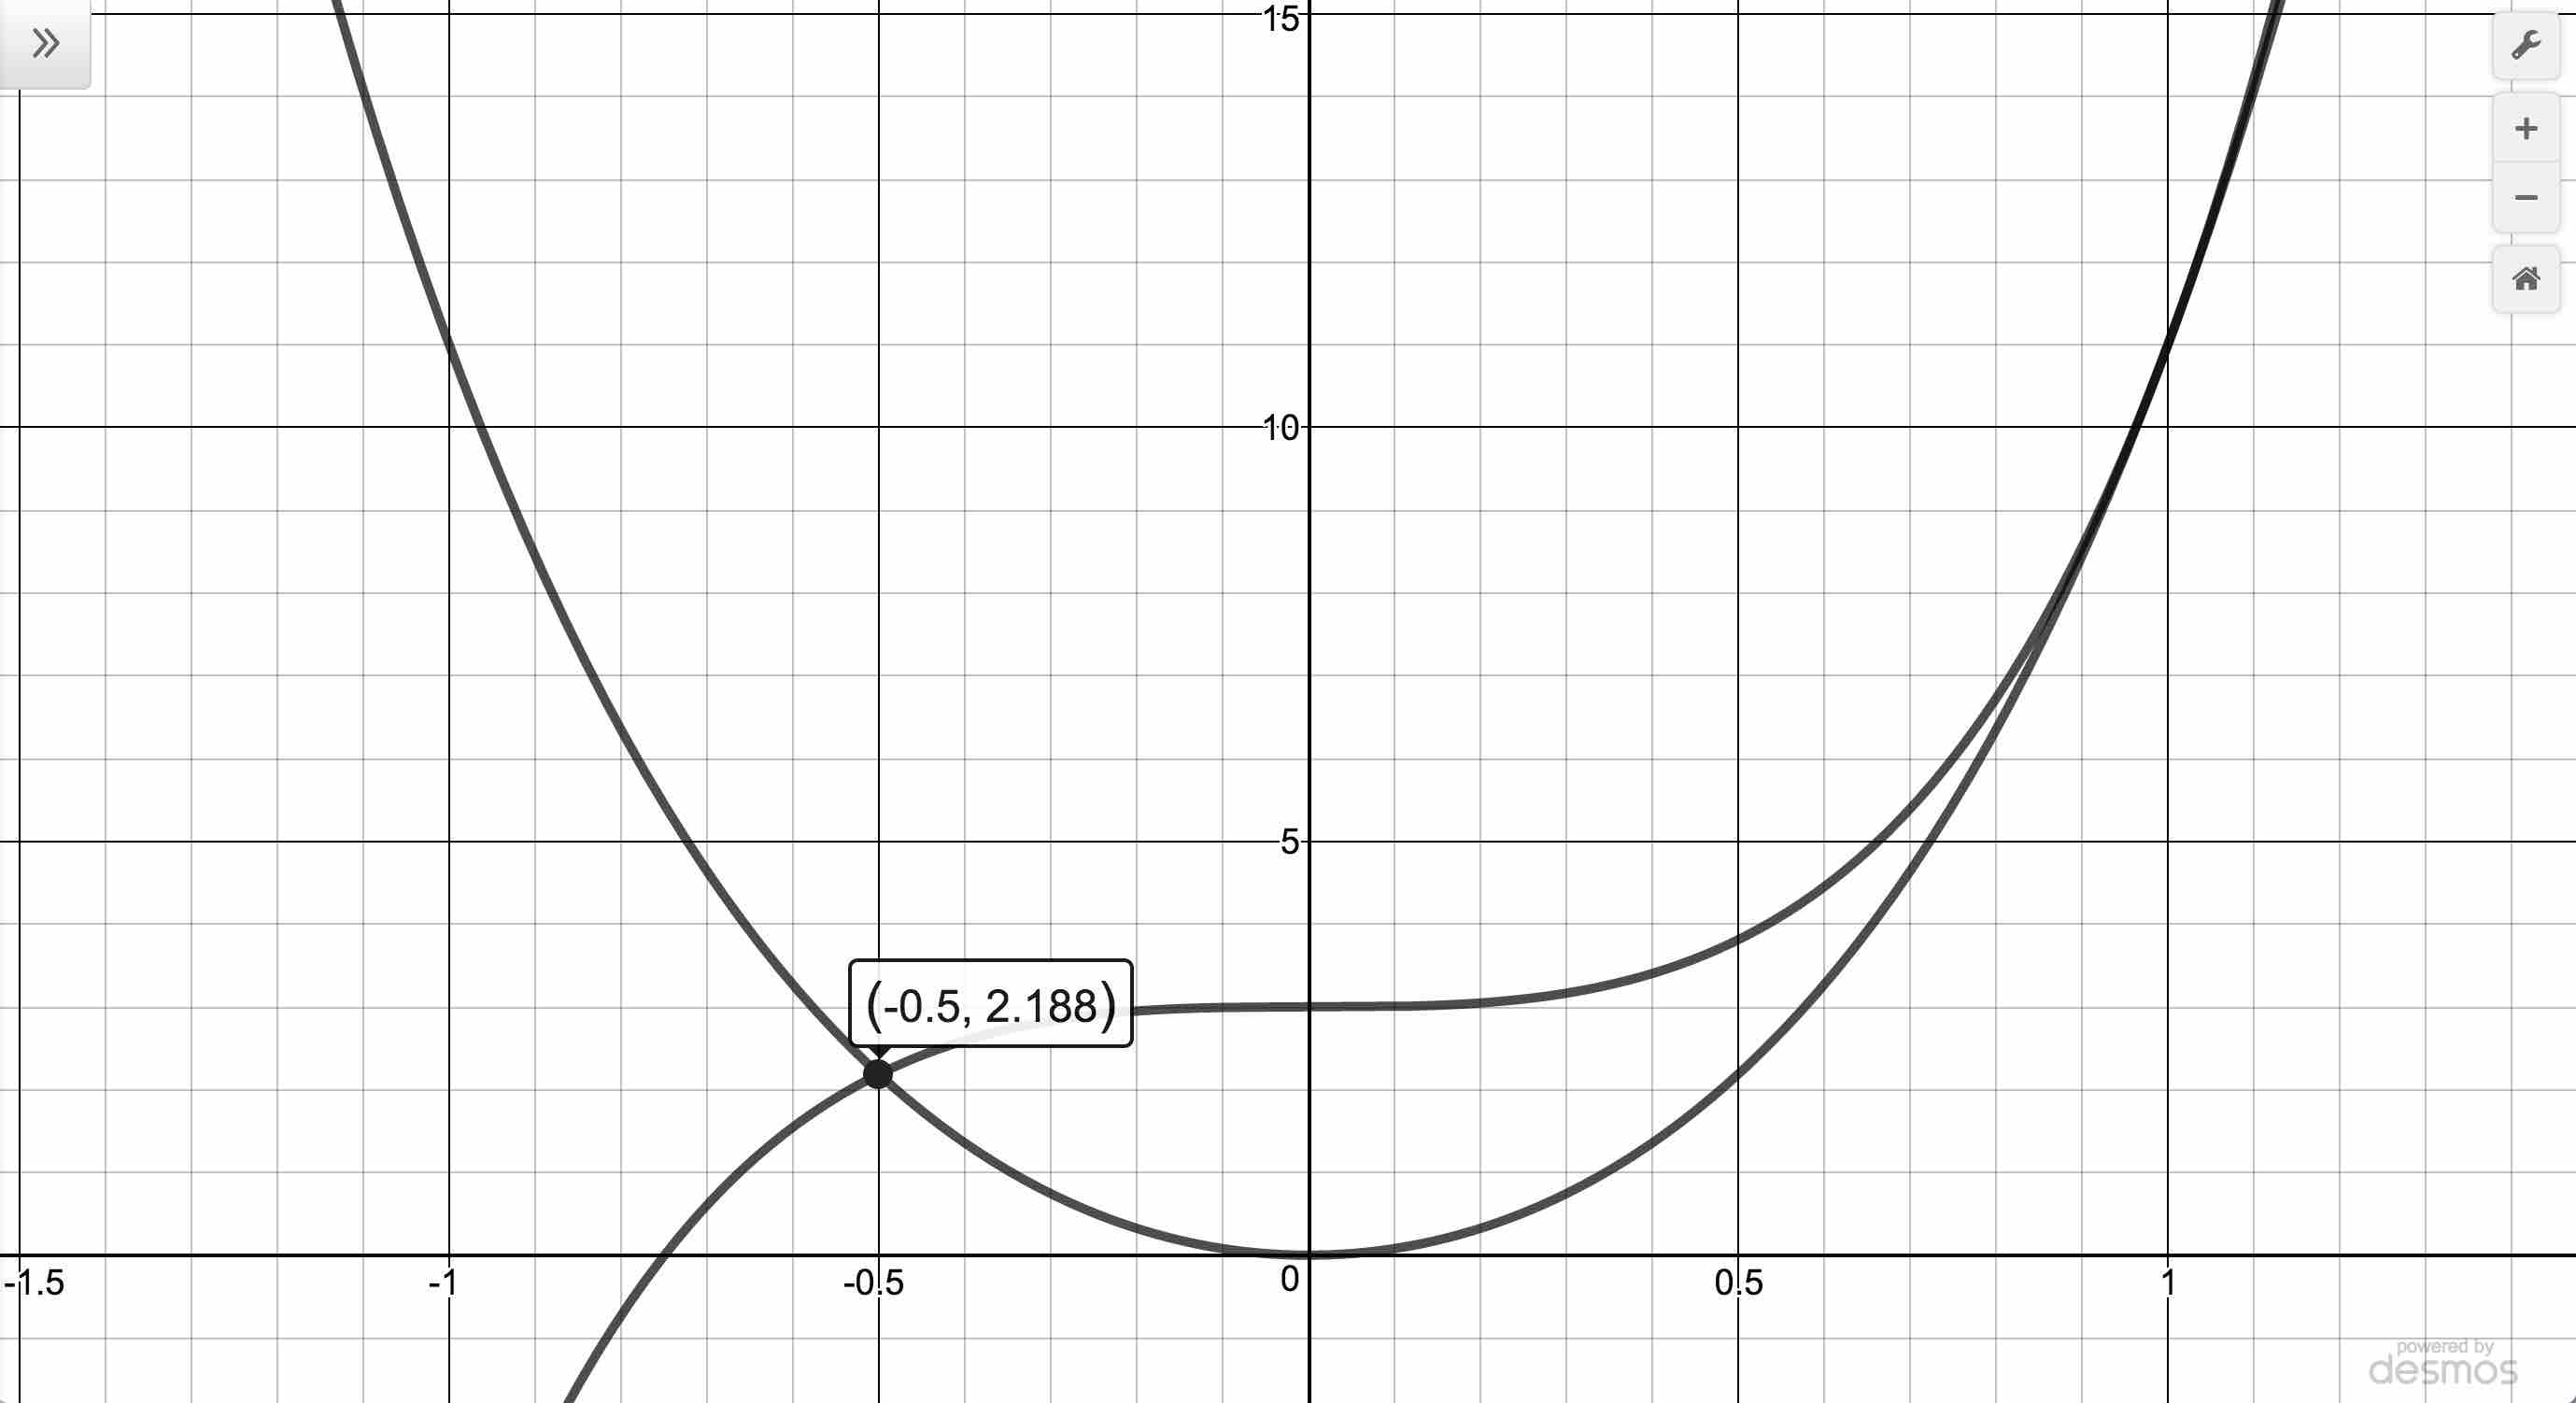
\includegraphics[width = 3in, height=2in]{./RealZerosGraphics/RealZerosEx03a.jpg}  &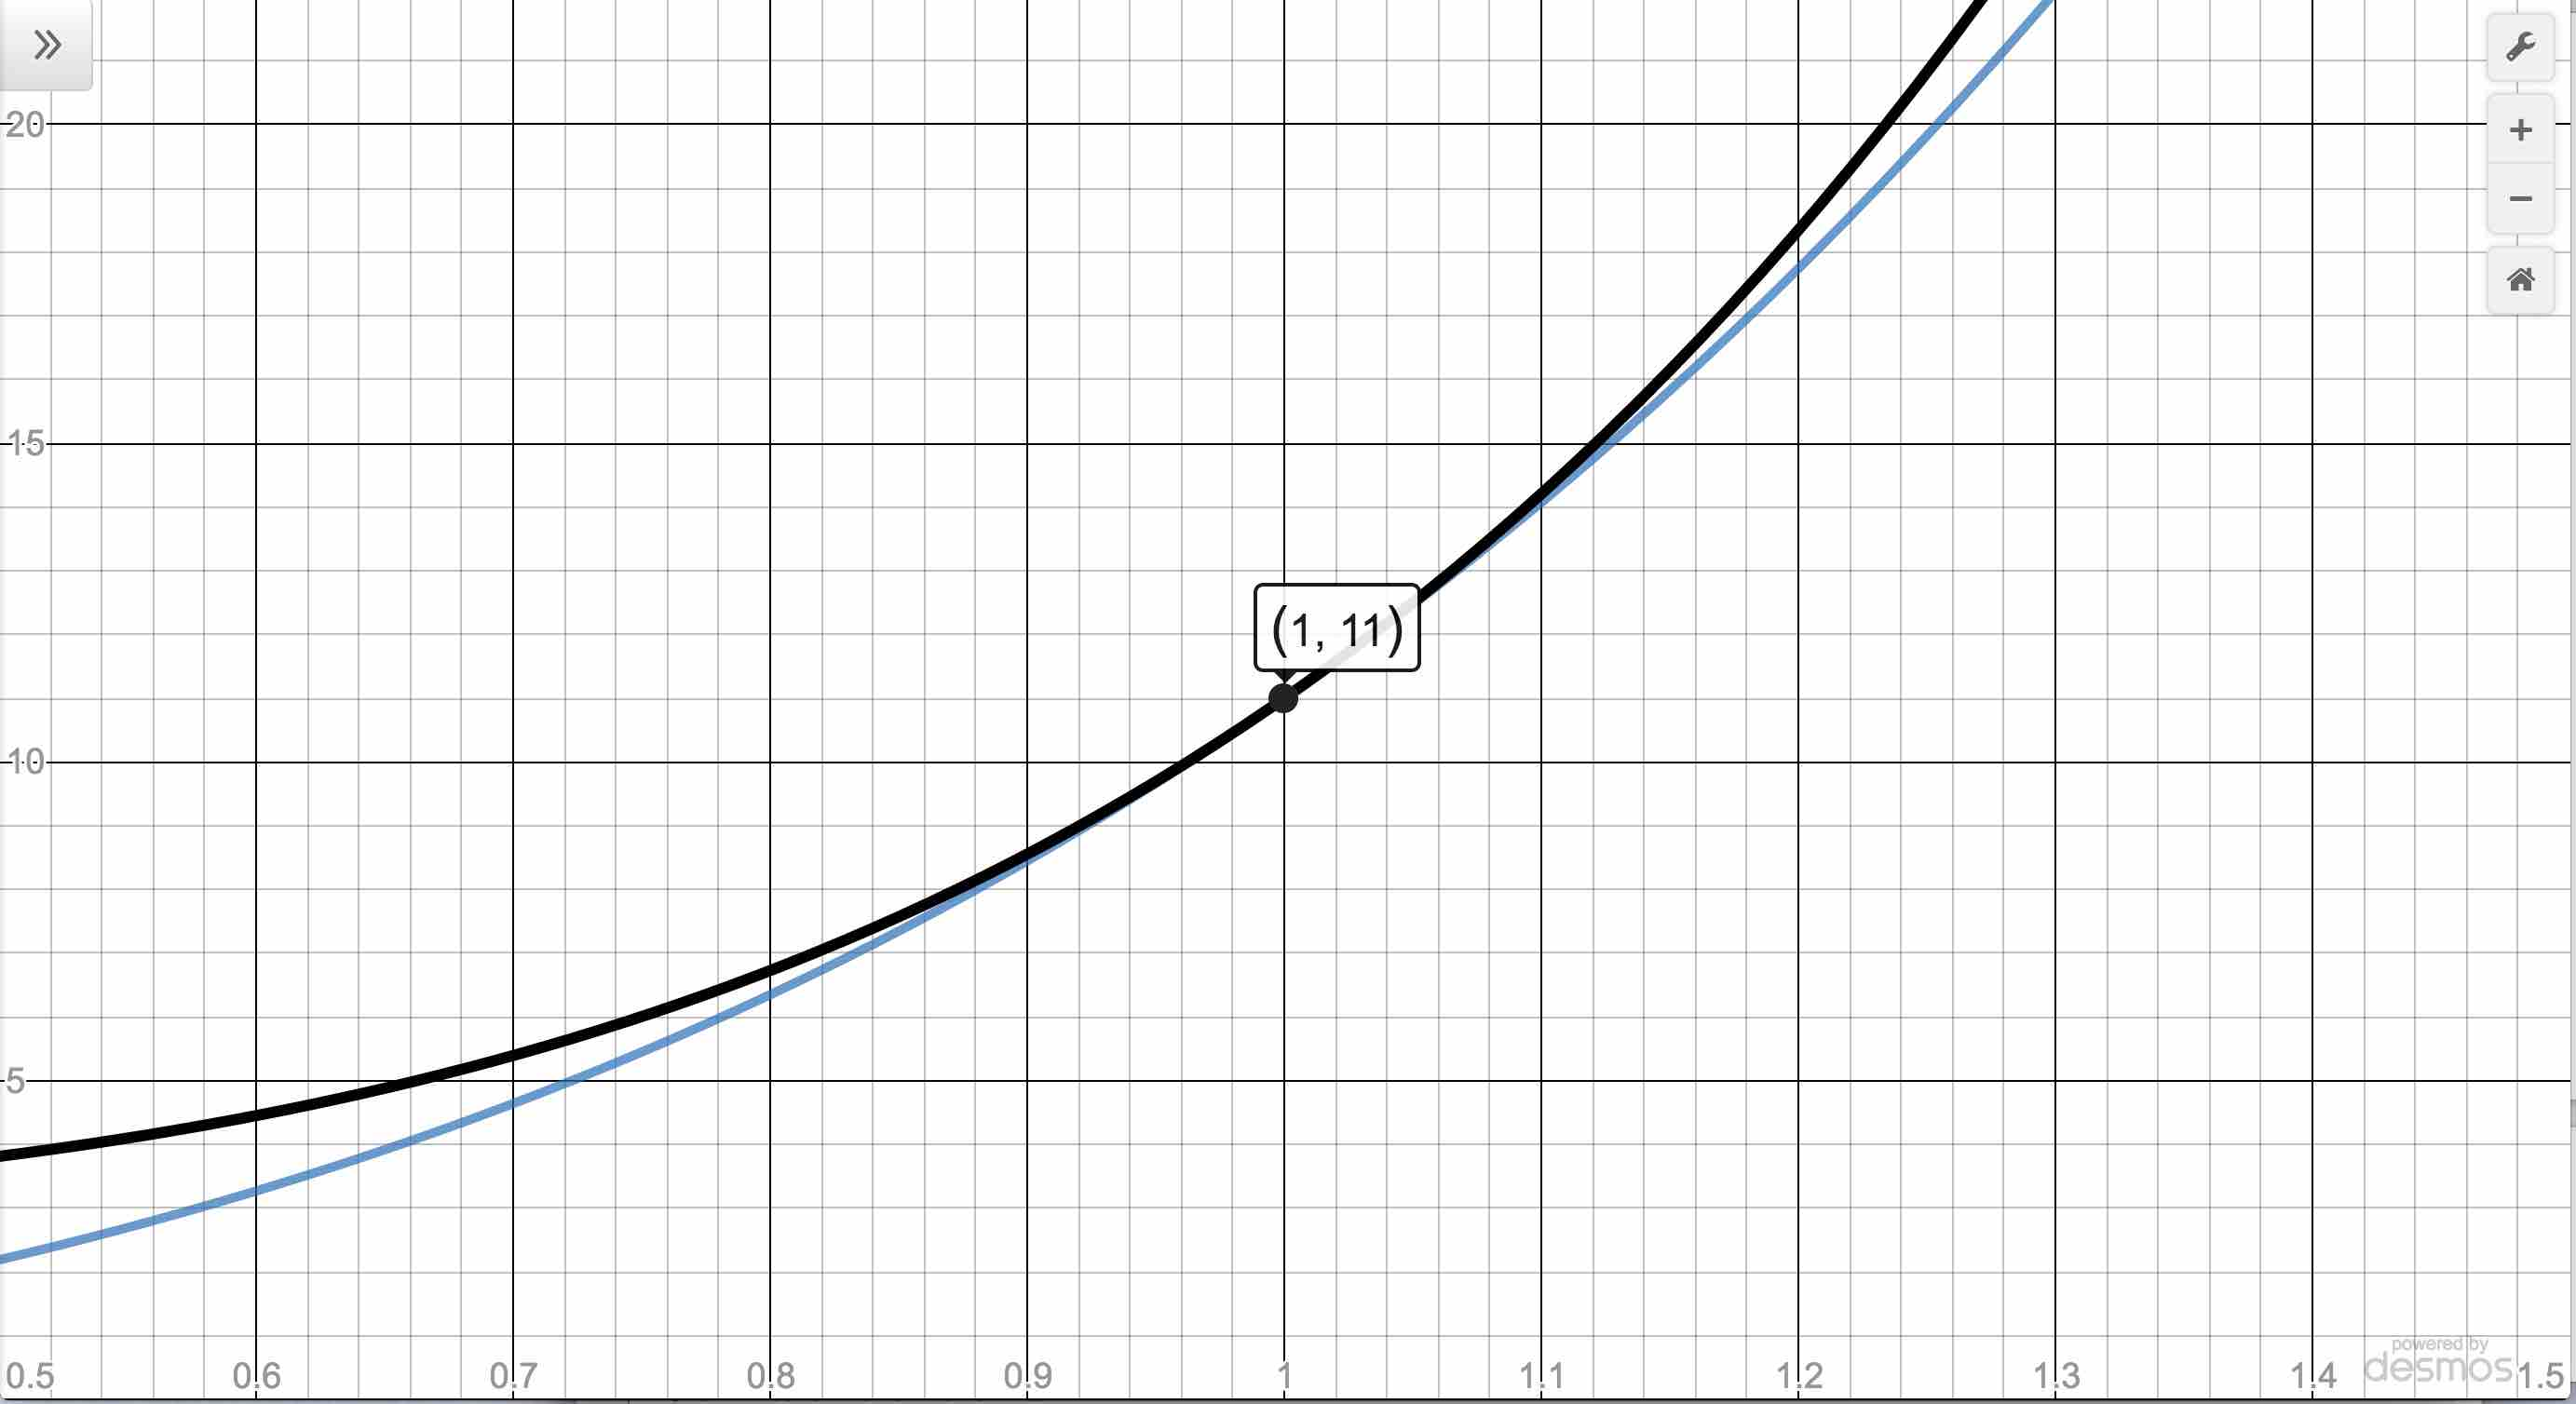
\includegraphics[width = 3in, height=2in]{./RealZerosGraphics/RealZerosEx03b.jpg}

\end{tabular}
\end{center} 

\qed
\end{enumerate}

\end{ex}

Note that we could have used end behavior and the concept of multiplicity to create the sign diagram used in Example \ref{polyeqineqexample} as follows.  We know the end behavior of $p(x) = 2x^5-3x^4+6x^3-8x^2+3$ matches that of $y = 2x^5$ which means $\ds{\lim_{x \rightarrow -\infty} p(x) = -\infty}$.  This means for the interval $\left(-\infty, -\frac{1}{2}\right)$, $p(x) < 0$ or $(-)$. From our work finding the zeros of $p$, we can deduce the multiplicity of the zero $x = -\frac{1}{2}$ is $1$ which means the graph of $y = p(x)$ crosses through the $x$-axis at $\left( -\frac{1}{2}, 0 \right)$, hence, changing sign from $(-)$ to $(+)$.  Finally, we can deduce the multiplicity of the zero $x = 1$ is $2$ which means the graph of $y = p(x)$ rebounds here, meaning the sign of $p(x)$ for $x > 1$ is $(+)$.  This matches the end behavior, since $\ds{\lim_{x \rightarrow \infty} p(x) = \infty}$.  The reader is encouraged to tackle any given problem using whatever tools are comfortable and convenient, but it also never hurts to think outside the box and revisit a problem from a variety of perspectives.

Next up is an application problem torn  from page \pageref{LCDmaxprofit} in the Exercises of Section \ref{GraphsofPolynomials}.

\begin{ex} Suppose the profit $P$, in \textit{thousands} of dollars, from producing and selling $x$ \textit{hundred} LCD TVs is given by  $P(x)=-5x^3+35x^2-45x-25$, $0 \leq x \leq 10.07$.  How many TVs should be produced to make a profit?  Check your answer using a graphing utility.

\smallskip

{\bf Solution.}  To `make a profit' means to solve $P(x) = -5x^3+35x^2-45x-25 > 0$, which we do analytically using a sign diagram.  To simplify things, we first factor out the $-5$ common to all the coefficients to get $-5\left(x^3 - 7x^2+9x-5\right) > 0$, so we can just focus on finding the zeros of $f(x) = x^3-7x^2+9x+5$.  The possible rational zeros of $f$ are $\pm 1$ and $\pm 5$, and going through the usual computations, we find $x=5$ is the only rational zero.  Using this, we factor $f(x) = x^3-7x^2+9x+5 = (x-5) \left(x^2-2x-1\right)$, and we find the remaining zeros by applying the Quadratic Formula to $x^2-2x-1 = 0$.  We find three real zeros,  $x=1-\sqrt{2} = -0.414 \ldots$,  $x = 1+\sqrt{2} = 2.414 \ldots$, and $x = 5$, of which only the last two fall in the applied domain of $[0, 10.07]$.  We choose $x=0$, $x=3$ and $x=10.07$ as our test values and plug them into the function $P(x)=-5x^3+35x^2-45x-25$ (not $f(x) =x^3 - 7x^2+9x-5$) to get the sign diagram below.

\begin{center}

\begin{mfpic}[10]{-5}{5}{-2}{2}
\polyline{(-5,0),(5,0)}
\point[3pt]{(-5,0), (5,0)}
\xmarks{-2,2}
\arrow \polyline{(-5,-1.5),(-5,-0.5)}
\arrow \polyline{(0,-1.5),(0,-0.5)}
\arrow \polyline{(5,-1.5),(5,-0.5)}
\tlpointsep{4pt}
\axislabels {x}{{\scriptsize $1+\sqrt{2} \hspace{7pt}$} -2, {\scriptsize $5$} 2}
\tlabel[cc](-5,1){$(-)$}
\tlabel[cc](-2,1){$0$}
\tlabel[cc](0,1){$(+)$}
\tlabel[cc](2,1){$0$}
\tlabel[cc](-5,-2.25){$0$}
\tlabel[cc](0,-2.25){$3$}
\tlabel[cc](5,-2.25){$10.07$}
\tlabel[cc](5,1){$(-)$}
\end{mfpic} 

\end{center}

We see immediately that $P(x)>0$ on $(1+\sqrt{2},5)$.  Since $x$ measures the number of TVs in \textit{hundreds}, $x = 1 + \sqrt{2}$ corresponds to $241.4\ldots$ TVs.  Since we can't produce a fractional part of a TV, we need to choose between producing 241 and 242 TVs.  From the sign diagram, we see that $P(2.41) < 0$ but $P(2.42)>0$ so, in this case we take the next \textit{larger} integer value and set the minimum production to 242 TVs.  At the other end of the interval, we have $x=5$ which corresponds to $500$ TVs.  Here, we take the next \textit{smaller} integer value, $499$ TVs to ensure that we make a profit.  Hence, in order to make a profit, at least 242, but no more than 499 TVs need to be produced.  We graph $y = P(x)$ below using a graphing utility and see $P(x) > 0$ between $x \approx 2.414$ and $x = 5$, as predicted.
\begin{center}

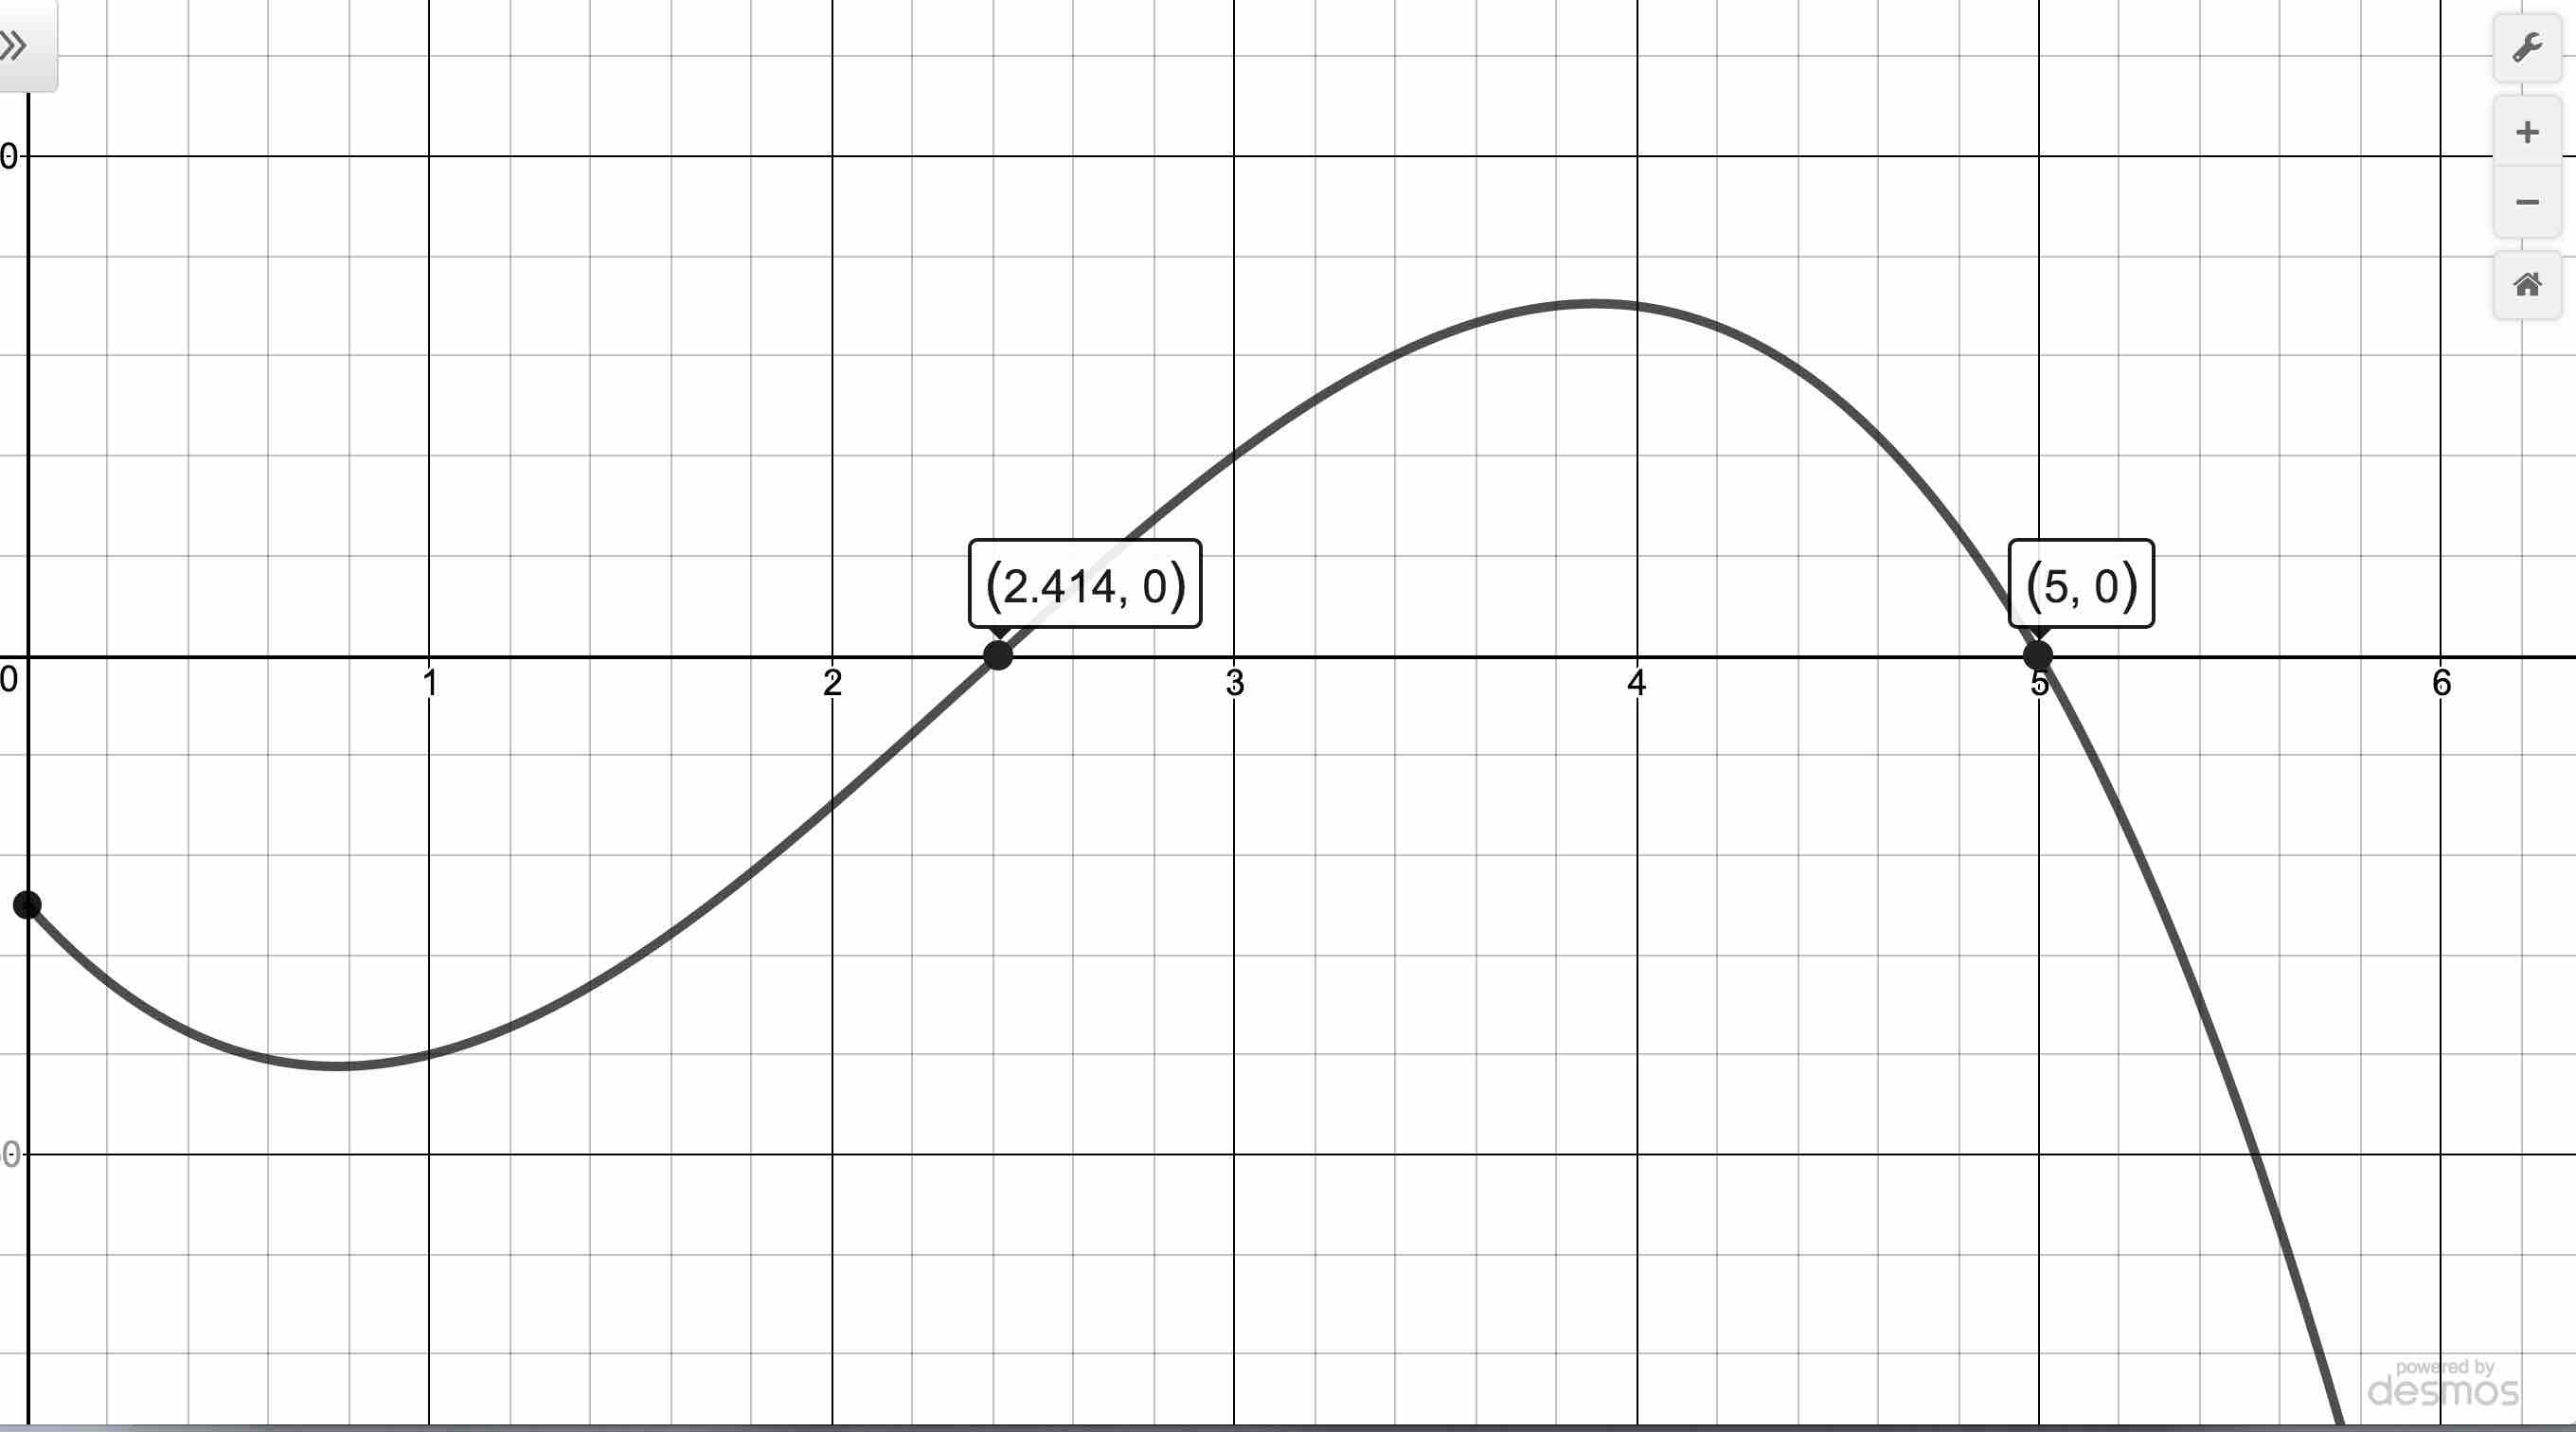
\includegraphics[width = 4in]{./RealZerosGraphics/RealZerosEx04.jpg}

\end{center}  

 \qed

\end{ex}


It would be a sin of omission if the authors left the reader with the impression that the theory in this section is compete in that given \textit{any} polynomial function, provided here are the tools to find all of its real zeros exactly.  The reality is this couldn't be further from the truth.  In general, no matter how many theorems you throw at a polynomial, it may well be impossible to express its zeros exactly.  The polynomial $f(x) = x^5-x-1$ is one such beast.\footnote{See this \href{http://en.wikipedia.org/wiki/Galois_theory}{\underline{page}}.}  According to Descartes' Rule of Signs, $f$ has exactly one positive real zero, and it could have two negative real zeros, or none at all.  The Rational Zeros Test gives us $\pm 1$ as rational zeros to try but neither of these work since $f(1) = f(-1) = -1$.  If we try the substitution technique we used in Example \ref{usubex}, we find $f(x)$ has three terms, but the exponent on the $x^5$ isn't exactly twice the exponent on $x$.  How could we go about approximating the positive zero?   We use the \index{Bisection Method} \textbf{Bisection Method}.  

\phantomsection
\label{bisectionmethod}

The first step in the Bisection Method is to find an interval on which $f$ changes sign.  We know $f(1) = -1$ and we find $f(2) = 29$.  By the Intermediate Value Theorem, we know that the zero of $f$ lies in the interval $[1,2]$.  Next, we `bisect' this interval by finding the midpoint,  $1.5$.  We compute  $f(1.5)\approx 5.09$.  Once again, the Intermediate Value Theorem guarantees our zero is between $1$ and $1.5$, since $f$ changes sign on this interval.  Now, we `bisect' the interval $[1,1.5]$ and find $f(1.25) \approx 0.80$, so now we have the zero between $1$ and $1.25$.  Bisecting $[1,1.25]$, we find $f(1.125) \approx -0.32$, which means the zero of $f$ is between $1.125$ and $1.25$.  We continue in this fashion until we have `sandwiched' the zero between two numbers whose digits agree to a desired amount.\footnote{We ask you to approximate this zero to three decimal places using the Bisection Method  in Exercise \ref{bisectionexercise}.} You can think of the Bisection Method as reversing the sign diagram process:  instead of finding the zeros and checking the sign of $f$ using test values, we are using test values to determine where the signs switch to find the zeros.  It is a slow and tedious, yet fool-proof, method for \textit{approximating} a real zero when the other analytical methods fail us.  


\newpage

\subsection{Exercises}

\documentclass{ximera}

\begin{document}
	\author{Stitz-Zeager}
	\xmtitle{TITLE}
\mfpicnumber{1} \opengraphsfile{ExercisesforRealZeros} % mfpic settings added 


In Exercises \ref{prelimpolystufffirst} - \ref{prelimpolystufflast}, for the given polynomial:

\begin{itemize}
\item  Use Cauchy's Bound to find an interval containing all of the real zeros.
\item  Use the Rational Zeros Theorem to make a list of possible rational zeros.
\item  Use Descartes' Rule of Signs to list the possible number of positive and negative real zeros, counting multiplicities.
\end{itemize}


\begin{multicols}{2}
\begin{enumerate}

\item $f(x) = x^{3} - 2x^{2} - 5x + 6$ \label{prelimpolystufffirst}
\item $f(x) = x^{4} + 2x^{3} - 12x^{2} - 40x - 32$

\setcounter{HW}{\value{enumi}}
\end{enumerate}
\end{multicols}

\begin{multicols}{2}
\begin{enumerate}
\setcounter{enumi}{\value{HW}}

\item $p(z) = z^{4} - 9z^{2} - 4z + 12$
\item $p(z) = z^{3} + 4z^{2} - 11z + 6$

\setcounter{HW}{\value{enumi}}
\end{enumerate}
\end{multicols}

\begin{multicols}{2}
\begin{enumerate}
\setcounter{enumi}{\value{HW}}

\item $g(t) = t^{3} - 7t^{2} + t - 7$
\item $g(t) = -2t^{3} + 19t^{2} - 49t + 20$

\setcounter{HW}{\value{enumi}}
\end{enumerate}
\end{multicols}

\begin{multicols}{2}
\begin{enumerate}
\setcounter{enumi}{\value{HW}}

\item $f(x) = -17x^{3} + 5x^{2} + 34x - 10$
\item $f(x) = 36x^{4} - 12x^{3} - 11x^{2} + 2x + 1$

\setcounter{HW}{\value{enumi}}
\end{enumerate}
\end{multicols}

\begin{multicols}{2}
\begin{enumerate}
\setcounter{enumi}{\value{HW}}

\item $p(z) = 3z^{3} + 3z^{2} - 11z - 10$
\item $p(z) = 2z^4+z^3-7z^2-3z+3$ \label{prelimpolystufflast}


\setcounter{HW}{\value{enumi}}
\end{enumerate}
\end{multicols}


In Exercises \ref{findrealzerosexerfirst} - \ref{findrealzerosexerlast}, find the real zeros of the polynomial using the techniques specified by your instructor.  State the multiplicity of each real zero.


\begin{multicols}{2}
\begin{enumerate}
\setcounter{enumi}{\value{HW}}

\item $f(x) = x^{3} - 2x^{2} - 5x + 6$ \label{findrealzerosexerfirst}
\item $f(x) = x^{4} + 2x^{3} - 12x^{2} - 40x - 32$

\setcounter{HW}{\value{enumi}}
\end{enumerate}
\end{multicols}

\begin{multicols}{2}
\begin{enumerate}
\setcounter{enumi}{\value{HW}}

\item $p(z) = z^{4} - 9z^{2} - 4z + 12$
\item $p(z) = z^{3} + 4z^{2} - 11z + 6$

\setcounter{HW}{\value{enumi}}
\end{enumerate}
\end{multicols}

\begin{multicols}{2}
\begin{enumerate}
\setcounter{enumi}{\value{HW}}

\item $g(t) = t^{3} - 7t^{2} + t - 7$
\item $g(t) = -2t^{3} + 19t^{2} - 49t + 20$

\setcounter{HW}{\value{enumi}}
\end{enumerate}
\end{multicols}

\begin{multicols}{2}
\begin{enumerate}
\setcounter{enumi}{\value{HW}}

\item $f(x) = -17x^{3} + 5x^{2} + 34x - 10$
\item $f(x) = 36x^{4} - 12x^{3} - 11x^{2} + 2x + 1$

\setcounter{HW}{\value{enumi}}
\end{enumerate}
\end{multicols}

\begin{multicols}{2}
\begin{enumerate}
\setcounter{enumi}{\value{HW}}

\item $p(z) = 3z^{3} + 3z^{2} - 11z - 10$
\item $p(z) = 2z^4+z^3-7z^2-3z+3$

\setcounter{HW}{\value{enumi}}
\end{enumerate}
\end{multicols}

\begin{multicols}{2}
\begin{enumerate}
\setcounter{enumi}{\value{HW}}

\item $g(t) = 9t^{3} - 5t^{2} - t$
\item $g(t) = 6t^{4} - 5t^{3} - 9t^{2}$

\setcounter{HW}{\value{enumi}}
\end{enumerate}
\end{multicols}

\begin{multicols}{2}
\begin{enumerate}
\setcounter{enumi}{\value{HW}}

\item $f(x) = x^4+2x^2 - 15$
\item $f(x) = x^4-9x^2+14$

\setcounter{HW}{\value{enumi}}
\end{enumerate}
\end{multicols}

\begin{multicols}{2}
\begin{enumerate}
\setcounter{enumi}{\value{HW}}

\item $p(z) = 3z^4-14z^2-5$
\item $p(z) = 2z^4-7z^2+6$

\setcounter{HW}{\value{enumi}}
\end{enumerate}
\end{multicols}

\begin{multicols}{2}
\begin{enumerate}
\setcounter{enumi}{\value{HW}}

\item $g(t) = t^6-3t^3-10$
\item $g(t) = 2t^6-9t^3+10$

\setcounter{HW}{\value{enumi}}
\end{enumerate}
\end{multicols}

\begin{multicols}{2}
\begin{enumerate}
\setcounter{enumi}{\value{HW}}

\item $f(x) = x^5-2x^4-4x+8$
\item $f(x) = 2x^5+3x^4-18x-27$ \label{findrealzerosexerlast}

\setcounter{HW}{\value{enumi}}
\end{enumerate}
\end{multicols}

\pagebreak

In Exercises \ref{realzeroswcalcfirst} - \ref{realzeroswcalclast}, use your calculator,\footnote{You \textit{can} do these without your calculator, but it may test your mettle!} to help you find the real zeros of the polynomial.  State the multiplicity of each real zero.

\begin{enumerate}
\setcounter{enumi}{\value{HW}}

\item $f(x) = x^{5} - 60x^{3} - 80x^{2} + 960x + 2304$ \label{realzeroswcalcfirst}
\item $f(x) = 25x^{5} - 105x^{4} + 174x^{3} - 142x^{2} + 57x - 9$
\item $f(x) = 90x^{4} - 399x^{3} + 622x^{2} - 399x + 90$ \label{realzeroswcalclast}

\setcounter{HW}{\value{enumi}}
\end{enumerate}

\begin{enumerate}
\setcounter{enumi}{\value{HW}}

\item Find the real zeros of $f(x) = x^{3} - \frac{1}{12}x^{2} - \frac{7}{72}x + \frac{1}{72}$ by first finding a polynomial $q(x)$ with integer coefficients such that $q(x) = N \cdot f(x)$ for some integer $N$.  (Recall that the Rational Zeros Theorem required the polynomial in question to have integer coefficients.) Show that $f$ and $q$ have the same real zeros.

\setcounter{HW}{\value{enumi}}
\end{enumerate}

In Exercises \ref{polyequexerfirst} - \ref{polyequexerlast}, find the real solutions of the polynomial equation.  (See Example \ref{polyeqineqexample}.)

\begin{multicols}{2}
\begin{enumerate}
\setcounter{enumi}{\value{HW}}

\item  $9x^{3} = 5x^{2} + x$  \label{polyequexerfirst} 
\item $9x^{2}+5x^{3}= 6x^{4}$  

\setcounter{HW}{\value{enumi}}
\end{enumerate}
\end{multicols}

\begin{multicols}{2}
\begin{enumerate}
\setcounter{enumi}{\value{HW}}

\item $z^{3} + 6 = 2z^{2} + 5z$ 
\item $z^{4} + 2z^{3} = 12z^{2} + 40z + 32$ 

\setcounter{HW}{\value{enumi}}
\end{enumerate}
\end{multicols}


\begin{multicols}{2}
\begin{enumerate}
\setcounter{enumi}{\value{HW}}

\item $t^{3} - 7t^{2} = 7-t$ 
\item $2t^{3} = 19t^{2} - 49t + 20$ 

\setcounter{HW}{\value{enumi}}
\end{enumerate}
\end{multicols}

\begin{multicols}{2}
\begin{enumerate}
\setcounter{enumi}{\value{HW}}

\item $x^{3} + x^{2} = \dfrac{11x + 10}{3}$ 
\item $x^4+2x^2 = 15$ 


\setcounter{HW}{\value{enumi}}
\end{enumerate}
\end{multicols}

\begin{multicols}{2}
\begin{enumerate}
\setcounter{enumi}{\value{HW}}

\item $14z^{2}+5=3z^{4}$  

\item $2z^5+3z^4 = 18z + 27$ \label{polyequexerlast}  

\setcounter{HW}{\value{enumi}}
\end{enumerate}
\end{multicols}


In Exercises \ref{polyinequexerfirst} - \ref{polyinequexerlast}, solve the polynomial inequality and state your answer using interval notation.



\begin{multicols}{2}
\begin{enumerate}
\setcounter{enumi}{\value{HW}}

\item $-2x^{3} + 19x^{2} - 49x + 20 > 0$ \label{polyinequexerfirst}
\item $x^{4} - 9x^{2} \leq 4x - 12$

\setcounter{HW}{\value{enumi}}
\end{enumerate}
\end{multicols}

\begin{multicols}{2}
\begin{enumerate}
\setcounter{enumi}{\value{HW}}

\item $(z - 1)^{2} \geq 4$
\item $4z^3 \geq 3z+1$

\setcounter{HW}{\value{enumi}}
\end{enumerate}
\end{multicols}

\begin{multicols}{2}
\begin{enumerate}
\setcounter{enumi}{\value{HW}}

\item $t^4 \leq 16+4t-t^3$
\item $3t^2 + 2t < t^4$

\setcounter{HW}{\value{enumi}}
\end{enumerate}
\end{multicols}

\begin{multicols}{2}
\begin{enumerate}
\setcounter{enumi}{\value{HW}}

\item $\dfrac{x^3+2 x^2}{2} < x+2$
\item $\dfrac{x^3+20x}{8} \geq x^2 + 2$

\setcounter{HW}{\value{enumi}}
\end{enumerate}
\end{multicols}

\begin{multicols}{2}
\begin{enumerate}
\setcounter{enumi}{\value{HW}}

\item $2z^4>5z^2+3$
\item $z^6 + z^3 \geq 6$ \label{polyinequexerlast}

\setcounter{HW}{\value{enumi}}
\end{enumerate}
\end{multicols}


\newpage

In Exercises \ref{polyineqfromgraphfirst} - \ref{polyineqfromgraphlast}, use the the graph of the given polynomial function to  solve the stated inequality.

\begin{multicols}{2}
\begin{enumerate}
\setcounter{enumi}{\value{HW}}

\item  \label{polyineqfromgraphfirst} Solve $f(x) < 0$. 

\begin{mfpic}[10]{-7}{7}{-6}{6}
\axes
\tlabel[cc](7,-0.5){\scriptsize $x$}
\tlabel[cc](0.5,6){\scriptsize $y$}
\tlabel[cc](-4.5, 0.75){\scriptsize $(-6,0)$}
\tlabel[cc](5, 0.75){\scriptsize $(6,0)$}
\tlabel[cc](1, 0.75){\scriptsize $(0,0)$}
\point[4pt]{(-6,0),(0,0),(6,0)}
\xmarks{-6 step 1 until 6}
\tiny
\tlpointsep{4pt}
\axislabels {x}{{$-6 \hspace{6pt}$} -6, {$-5 \hspace{6pt}$} -5, {$-4 \hspace{6pt}$} -4, {$-3 \hspace{6pt}$} -3, {$-2 \hspace{6pt}$} -2, {$-1 \hspace{6pt}$} -1, {$1$} 1, {$2$} 2, {$3$} 3, {$4$} 4, {$5$} 5, {$6$} 6}
\normalsize
\penwd{1.25pt}
\arrow \reverse \arrow \function{-7,7,0.1}{((x**3) - 36*x)/20}
\tcaption{$y = f(x)$}
\end{mfpic}

\vfill

\columnbreak

\item Solve $g(t) > 0$.


\begin{mfpic}[20][20]{-3}{3}{-2}{5}
\axes
\tlabel[cc](3,-0.5){\scriptsize $t$}
\tlabel[cc](0.25,5){\scriptsize $y$}
\tlabel[cc](-1.75, 0.3){\scriptsize $(-2,0)$}
\tlabel[cc](0.5, 0.3){\scriptsize $(0,0)$}
\point[4pt]{(-2,0), (0,0)}
\xmarks{-2,-1, 1, 2}
\tiny
\tlpointsep{4pt}
\axislabels {x}{{$-2 \hspace{6pt}$} -2, {$-1 \hspace{6pt}$} -1, {$1$} 1, {$2$} 2}
\normalsize
\penwd{1.25pt}
\arrow \reverse \arrow \function{-3,0.3,0.1}{x*((x + 2)**3)}
\tcaption{$y = g(t)$ }
\end{mfpic}


\setcounter{HW}{\value{enumi}}
\end{enumerate}
\end{multicols}


\begin{multicols}{2}
\begin{enumerate}
\setcounter{enumi}{\value{HW}}

\item  Solve $p(z) \geq 0$ 

\begin{mfpic}[20][10]{-3}{3}{-4}{4}
\axes
\tlabel[cc](3,-0.5){\scriptsize $z$}
\tlabel[cc](0.25,4){\scriptsize $y$}
\tlabel[cc](-2, 0.75){\scriptsize $(-1,0)$}
\tlabel[cc](2, 0.75){\scriptsize $(2,0)$}
\point[4pt]{(2,0), (-1,0)}
\xmarks{-2,-1,1,2}
\tiny
\tlpointsep{4pt}
\axislabels {x}{{$-2 \hspace{6pt}$} -2, {$-1 \hspace{6pt}$} -1, {$1$} 1, {$2$} 2}
\normalsize
\penwd{1.25pt}
\arrow \reverse \arrow \function{-1.70,3.45,0.1}{(-0.4)*((x-2)**2)*(x+1)}
\tcaption{$y = p(z)$}
\end{mfpic}

\vfill

\columnbreak




\item Solve $f(x) < 0$.


\begin{mfpic}[20][10]{-2}{4}{-4}{4}
\axes
\tlabel[cc](4,-0.5){\scriptsize $x$}
\tlabel[cc](0.25,4){\scriptsize $y$}
\tlabel[cc](-0.75, 0.75){\scriptsize $\left(-\frac{1}{2},0 \right)$}
\tlabel[cc](2.5, 0.75){\scriptsize $(3,0)$}
\point[4pt]{(-0.5,0), (3,0)}
\xmarks{-1,1,2,3}
\tiny
\tlpointsep{4pt}
\axislabels {x}{ {$1$} 1, {$2$} 2, {$3$} 3}
\normalsize
\penwd{1.25pt}
\arrow \reverse \arrow \function{-1.5,3.3,0.1}{(0.5)*((x+0.5)**2)*(x-3)}
\tcaption{$y = f(x)$ }
\end{mfpic}

\setcounter{HW}{\value{enumi}}
\end{enumerate}
\end{multicols}


\begin{multicols}{2}
\begin{enumerate}
\setcounter{enumi}{\value{HW}}

\item Solve $F(s) \leq 0$.  

\begin{mfpic}[20][10]{-3}{3}{-5}{5}
\axes
\tlabel[cc](3,-0.5){\scriptsize $s$}
\tlabel[cc](0.25,5){\scriptsize $y$}
\tlabel[cc](-2, -0.75){\scriptsize $(-2,0)$}
\tlabel[cc](0.5, 0.75){\scriptsize $(0,0)$}
\point[4pt]{(-2,0), (0,0)}
\xmarks{-2,-1,1,2}
\tiny
\tlpointsep{4pt}
\axislabels {x}{ {$1$} 1, {$2$} 2}
\normalsize
\penwd{1.25pt}
\arrow \reverse \arrow \function{-3,0.65,0.1}{0-x*((x + 2)**2)}
\tcaption{$y = F(s)$}
\end{mfpic}



\vfill

\columnbreak

\item \label{polyineqfromgraphlast} Solve $G(t) \geq 0$.

\begin{mfpic}[20][10]{-3}{3}{-5}{5}
\axes
\tlabel[cc](-2, 0.75){\scriptsize $(-2,0)$}
\tlabel[cc](0.5, -0.75){\scriptsize $(0,0)$}
\tlabel[cc](3,-0.5){\scriptsize $t$}
\tlabel[cc](0.25,5){\scriptsize $y$}
\point[4pt]{(-2,0), (0,0)}
\xmarks{-2,-1,1,2}
\tiny
\tlpointsep{4pt}
\axislabels {x}{  {$2$} 2}
\normalsize
\penwd{1.25pt}
\arrow \reverse \arrow \function{-2.45,0.85,0.1}{(x**3)*((x + 2)**2)}
\tcaption{$y = G(t)$}
\end{mfpic}


\setcounter{HW}{\value{enumi}}
\end{enumerate}
\end{multicols}



\begin{enumerate}
\setcounter{enumi}{\value{HW}}

\item Use the Intermediate Value Theorem, Theorem \ref{IVT} to prove that $f(x) = x^{3} - 9x + 5$ has a real zero in each of the following intervals: $[-4, -3], [0, 1]$ and $[2, 3]$.

\item  Use the concepts of End Behavior and the Intermediate Value Theorem to prove any odd-degree polynomial function with real number coefficients has at least one real zero.

\item Find an even-degree polynomial function with real number coefficients which has no real zeros.

\item  \label{bisectionexercise} Continue  the Bisection Method as introduced on  \pageref{bisectionmethod} to approximate the real zero of $f(x) = x^5-x-1$ to three decimal places.

\item  \label{sqrt2isirrationalexercise} In this exercise, we prove $\sqrt{2}$ is an irrational number and approximate its value.  Let $f(x) = x^2-2$.

\begin{enumerate} 

\item Use Decartes' Rule of Signs to prove $f$ has exactly one positive real zero.

 \item Use the Intermediate Value Theorem to prove $f$ has a zero in $[1,2]$.

\item \label{sqrt2isirrationalexercise}  Use the Rational Zeros Theorem to prove $f$ has no rational zeros.

\item  Use the Bisection Method (see  \pageref{bisectionmethod}) to approximate the zero of $f$ on $[1,2]$ to three decimal places.

\end{enumerate}

\item  Generalize the argument given in Exercise \ref{sqrt2isirrationalexercise} to prove:

\begin{enumerate}

\item If $N$ is not the perfect square of an integer, then $\sqrt{N}$ is irrational. (HINT: Consider $f(x) = x^2-N$.)

\item  For natural numbers $n \geq 2$, if $N$ is not the perfect $n^{\text{th}}$ power of an integer, then $\sqrt[n]{N}$ is irrational. (HINT: Consider $f(x) = x^n-N$.)

\end{enumerate}

\item  In Example \ref{boxnotopex} in Section \ref{GraphsofPolynomials}, a box with no top is constructed from a $10$ inch $\times$ $12$ inch piece of cardboard by cutting out congruent squares from each corner of the cardboard and then folding the resulting tabs.  We determined the volume of that box (in cubic inches) is given by  the function$V(x) = 4x^3-44x^2+120x$, where $x$ denotes the length of the side of the square which is removed from each corner (in inches), $0 < x < 5$.  Solve the inequality $V(x) \geq 80$ analytically and interpret your answer in the context of that example.

\item  From Exercise \ref{newportaboycost} in Section \ref{GraphsofPolynomials}, $C(x) = .03x^{3} - 4.5x^{2} + 225x + 250$, for $x \geq 0$ models the cost, in dollars, to produce $x$ PortaBoy game systems. If the production budget is $\$5000$, find the number of game systems which can be produced and still remain under budget.

\item Let $f(x) = 5x^{7} - 33x^{6} + 3x^{5} - 71x^{4} - 597x^{3} + 2097x^{2} - 1971x + 567$.  With the help of your classmates, find the $x$- and $y$- intercepts of the graph of $f$.  Find the intervals on which the function is increasing, the intervals on which it is decreasing and the local extrema.  Sketch the graph of $f$, using more than one picture if necessary to show all of the important features of the graph.  

\item With the help of your classmates, create a list of five polynomials with different degrees whose real zeros cannot be found using any of the techniques in this section.

\setcounter{HW}{\value{enumi}}
\end{enumerate}
 



\newpage

\subsection{Answers}

\begin{enumerate}

\item For $f(x) = x^{3} - 2x^{2} - 5x + 6$
\begin{itemize}
\item  All of the real zeros lie in the interval $[-7,7]$
\item  Possible rational zeros are $\pm 1$, $\pm 2$, $\pm 3$, $\pm 6$
\item  There are 2 or 0 positive real zeros;  there is 1 negative real zero
\end{itemize}

\item For  $f(x) = x^{4} + 2x^{3} - 12x^{2} - 40x - 32$
\begin{itemize}
\item  All of the real zeros lie in the interval $[-41,41]$
\item  Possible rational zeros are $\pm 1$, $\pm 2$, $\pm 4$, $\pm 8$, $\pm 16$, $\pm 32$
\item  There is 1 positive real zero;  there are 3 or 1 negative real zeros
\end{itemize}

\item For  $p(z) = z^{4} - 9z^{2} - 4z + 12$
\begin{itemize}
\item  All of the real zeros lie in the interval $[-13,13]$
\item  Possible rational zeros are $\pm 1$, $\pm 2$, $\pm 3$, $\pm 4$, $\pm 6$, $\pm 12$
\item  There are 2 or 0 positive real zeros;  there are 2 or 0 negative real zeros
\end{itemize}

\item For  $p(z) = z^{3} + 4z^{2} - 11z + 6$
\begin{itemize}
\item  All of the real zeros lie in the interval $[-12,12]$
\item  Possible rational zeros are $\pm 1$, $\pm 2$, $\pm 3$, $\pm 6$
\item  There are 2 or 0 positive real zeros;  there is 1 negative real zero
\end{itemize}

\item For   $g(t) = t^{3} - 7t^{2} + t - 7$
\begin{itemize}
\item  All of the real zeros lie in the interval $[-8,8]$
\item  Possible rational zeros are $\pm 1$, $\pm 7$
\item  There are 3 or 1 positive real zeros;  there are no negative real zeros
\end{itemize}

\item For   $g(t) = -2t^{3} + 19t^{2} - 49t + 20$
\begin{itemize}
\item  All of the real zeros lie in the interval $\left[-\frac{51}{2},\frac{51}{2} \right]$
\item  Possible rational zeros are  $\pm \frac{1}{2}$, $\pm 1$, $\pm 2$, $\pm \frac{5}{2}$, $\pm 4$, $\pm 5$, $\pm 10$, $\pm 20$ 
\item  There are 3 or 1 positive real zeros;  there are no negative real zeros
\end{itemize}

\item For   $f(x) = -17x^{3} + 5x^{2} + 34x - 10$
\begin{itemize}
\item  All of the real zeros lie in the interval $[-3,3]$
\item  Possible rational zeros are $\pm \frac{1}{17}$, $\pm \frac{2}{17}$, $\pm \frac{5}{17}$, $\pm \frac{10}{17}$, $\pm 1$, $\pm 2$, $\pm 5$, $\pm 10$
\item  There are 2 or 0 positive real zeros;  there is 1 negative real zero
\end{itemize}

\item For   $f(x) = 36x^{4} - 12x^{3} - 11x^{2} + 2x + 1$
\begin{itemize}
\item  All of the real zeros lie in the interval $\left[-\frac{4}{3},\frac{4}{3}\right]$
\item  Possible rational zeros are $\pm \frac{1}{36}$, $\pm \frac{1}{18}$, $\pm \frac{1}{12}$, $\pm \frac{1}{9}$, $\pm \frac{1}{6}$, $\pm \frac{1}{4}$, $\pm \frac{1}{3}$, $\pm \frac{1}{2}$, $\pm 1$
\item  There are 2 or 0 positive real zeros;  there are 2 or 0 negative real zeros
\end{itemize}

\item For   $p(z) = 3z^{3} + 3z^{2} - 11z - 10$
\begin{itemize}
\item  All of the real zeros lie in the interval $\left[-\frac{14}{3},\frac{14}{3}\right]$
\item  Possible rational zeros are $\pm \frac{1}{3}$, $\pm \frac{2}{3}$, $\pm \frac{5}{3}$, $\pm \frac{10}{3}$, $\pm 1$, $\pm 2$, $\pm 5$, $\pm 10$
\item  There is 1 positive real zero;  there are 2 or 0 negative real zeros
\end{itemize}

\item For   $p(z) = 2z^4+z^3-7z^2-3z+3$
\begin{itemize}
\item  All of the real zeros lie in the interval $\left[-\frac{9}{2},\frac{9}{2}\right]$
\item  Possible rational zeros are  $\pm \frac{1}{2}$, $\pm 1$,  $\pm \frac{3}{2}$, $\pm 3$
\item  There are 2 or 0 positive real zeros;  there are 2 or 0 negative real zeros
\end{itemize}


\item $f(x) = x^{3} - 2x^{2} - 5x + 6$ \\ $x = -2$, $x = 1$, $x = 3$ (each has mult. 1)
\item $f(x) = x^{4} + 2x^{3} - 12x^{2} - 40x - 32$ \\ $x = -2$ (mult. 3), $x = 4$ (mult. 1)


\item $p(z) = z^{4} - 9z^{2} - 4z + 12$ \\ $z = -2$ (mult. 2), $z = 1$ (mult. 1), $z = 3$ (mult. 1)
\item $p(z) = z^{3} + 4z^{2} - 11z + 6$ \\ $z = -6$ (mult. 1), $z = 1$ (mult. 2)

\item $g(t) = t^{3} - 7t^{2} + t - 7$ \\ $t = 7$ (mult. 1)
\item $g(t) = -2t^{3} + 19t^{2} - 49t + 20$ \\ $t = \frac{1}{2}$, $t = 4$, $t = 5$ (each has mult. 1)

\item $f(x) = -17x^{3} + 5x^{2} + 34x - 10$ \\ $x = \frac{5}{17}$, $x = \pm \sqrt{2}$ (each has mult. 1)
\item $f(x) = 36x^{4} - 12x^{3} - 11x^{2} + 2x + 1$ \\ $x = \frac{1}{2}$ (mult. 2), $x = -\frac{1}{3}$ (mult. 2)

\item $p(z) = 3z^{3} + 3z^{2} - 11z - 10$ \\ $z = -2$, $z = \frac{3 \pm \sqrt{69}}{6}$ (each has mult. 1)
\item $p(z) = 2z^4+z^3-7z^2-3z+3$ \\ $z = -1$, $z = \frac{1}{2}$, $z=\pm \sqrt{3}$ (each mult. 1)

\item $g(t) = 9t^{3} - 5t^{2} - t$ \\ $t = 0$, $t = \frac{5 \pm \sqrt{61}}{18}$ (each has mult. 1)
\item $g(t) = 6t^{4} - 5t^{3} - 9t^{2}$ \\ $t = 0$ (mult. 2), $t = \frac{5 \pm \sqrt{241}}{12}$ (each has mult. 1)

\item $f(x) = x^4+2x^2 - 15$ \\ $x = \pm \sqrt{3}$ (each has mult. 1)
\item $f(x) = x^4-9x^2+14$ \\ $x = \pm \sqrt{2}$, $x = \pm \sqrt{7}$ (each has mult. 1)

\item $p(z) = 3z^4-14z^2-5$ \\ $z = \pm \sqrt{5}$ (each has mult. 1)
\item $p(z)  = 2z^4-7z^2+6$ \\  $z = \pm \frac{\sqrt{6}}{2}$, $z = \pm \sqrt{2}$ (each has mult. 1)

\item $g(t) = t^6-3t^3-10$ \\ $t = \sqrt[3]{-2} = -\sqrt[3]{2}$, $t = \sqrt[3]{5}$ (each has mult. 1)
\item $g(t) = 2t^6-9t^3+10$ \\ $t =\frac{\sqrt[3]{20}}{2} $, $t = \sqrt[3]{2}$ (each has mult. 1)


\item $f(x) = x^5-2x^4-4x+8$ \\ $x = 2$, $x = \pm \sqrt{2}$ (each has mult. 1)
\item $f(x) = 2x^5+3x^4-18x-27$ \\ $x = -\frac{3}{2}$, $x = \pm \sqrt{3}$ (each has mult. 1)

\item $f(x) = x^{5} - 60x^{3} - 80x^{2} + 960x + 2304 $ \\ $x = -4$ (mult. 3), $x = 6$ (mult. 2)


\item $f(x) = 25x^{5} - 105x^{4} + 174x^{3} - 142x^{2} + 57x - 9$ \\ $x = \frac{3}{5}$ (mult. 2), $x = 1$ (mult. 3)

\item $f(x) = 90x^{4} - 399x^{3} + 622x^{2} - 399x + 90$ \\ $x = \frac{2}{3}$, $x = \frac{3}{2}$, $x = \frac{5}{3}$, $x = \frac{3}{5}$ (each has mult. 1)


\item We choose $q(x) = 72x^{3} - 6x^{2} - 7x + 1 = 72 \cdot f(x)$.  Clearly $f(x) = 0$ if and only if $q(x) = 0$ so they have the same real zeros.  In this case, $x = -\frac{1}{3}, \; x = \frac{1}{6} \;$ and $x = \frac{1}{4}$ are the real zeros of both $f$ and $q$.


\setcounter{HW}{\value{enumi}}
\end{enumerate}


\begin{multicols}{2}
\begin{enumerate}
\setcounter{enumi}{\value{HW}}

\item  $x = 0, \frac{5\pm \sqrt{61}}{18}$
\item  $x = 0, \frac{5 \pm \sqrt{241}}{12}$

\setcounter{HW}{\value{enumi}}
\end{enumerate}
\end{multicols}

\begin{multicols}{2}
\begin{enumerate}
\setcounter{enumi}{\value{HW}}

\item $z = -2,1,3$
\item $z=-2,4$

\setcounter{HW}{\value{enumi}}
\end{enumerate}
\end{multicols}


\begin{multicols}{2}
\begin{enumerate}
\setcounter{enumi}{\value{HW}}

\item $t=7$
\item $t = \frac{1}{2}, 4, 5$

\setcounter{HW}{\value{enumi}}
\end{enumerate}
\end{multicols}

\begin{multicols}{2}
\begin{enumerate}
\setcounter{enumi}{\value{HW}}

\item $x = -2, \frac{3 \pm \sqrt{69}}{6}$

\item $x = \pm \sqrt{3}$


\setcounter{HW}{\value{enumi}}
\end{enumerate}
\end{multicols}

\begin{multicols}{2}
\begin{enumerate}
\setcounter{enumi}{\value{HW}}

\item $z = \pm \sqrt{5}$

\item $z = -\frac{3}{2}, \pm \sqrt{3}$

\setcounter{HW}{\value{enumi}}
\end{enumerate}
\end{multicols}



\begin{multicols}{2}
\begin{enumerate}
\setcounter{enumi}{\value{HW}}

\item $(-\infty, \frac{1}{2}) \cup (4, 5)$
\item $\{-2\} \cup [1, 3]$

\setcounter{HW}{\value{enumi}}
\end{enumerate}
\end{multicols}

\begin{multicols}{2}
\begin{enumerate}
\setcounter{enumi}{\value{HW}}

\item $(-\infty, -1] \cup [3, \infty)$

\item $\left\{ -\dfrac{1}{2} \right\} \cup [1, \infty)$

\setcounter{HW}{\value{enumi}}
\end{enumerate}
\end{multicols}

\begin{multicols}{2}
\begin{enumerate}
\setcounter{enumi}{\value{HW}}

\item $[-2,2]$
\item $\left(-\infty, -1 \right) \cup \left(-1, 0 \right) \cup (2, \infty)$

\setcounter{HW}{\value{enumi}}
\end{enumerate}
\end{multicols}

\begin{multicols}{2}
\begin{enumerate}
\setcounter{enumi}{\value{HW}}


\item $(-\infty, -2) \cup \left(-\sqrt{2}, \sqrt{2} \right)$
\item $\{2 \} \cup [4,\infty)$

\setcounter{HW}{\value{enumi}}
\end{enumerate}
\end{multicols}

\begin{multicols}{2}
\begin{enumerate}
\setcounter{enumi}{\value{HW}}


\item $(-\infty, -\sqrt{3}) \cup (\sqrt{3}, \infty)$
\item $(-\infty, -\sqrt[3]{3}\,) \cup (\sqrt[3]{2}, \infty)$

\setcounter{HW}{\value{enumi}}
\end{enumerate}
\end{multicols}

\begin{multicols}{2}
\begin{enumerate}
\setcounter{enumi}{\value{HW}}

\item $f(x) < 0$ on $(-\infty, -6) \cup (0, 6)$

\item $g(t) > 0$ on $(-\infty, -2) \cup (0, \infty)$

\setcounter{HW}{\value{enumi}}
\end{enumerate}
\end{multicols}

\begin{multicols}{2}
\begin{enumerate}
\setcounter{enumi}{\value{HW}}

\item $p(z) \geq 0$ on $(-\infty, -1] \cup \{ 2\}$

\item $f(x) < 0$ on $\left( -\infty, -\frac{1}{2} \right) \cup \left(-\frac{1}{2}, 3 \right)$

\setcounter{HW}{\value{enumi}}
\end{enumerate}
\end{multicols}

\begin{multicols}{2}
\begin{enumerate}
\setcounter{enumi}{\value{HW}}

\item $F(s) \leq 0$ on $\{-2\} \cup [0, \infty)$

\item $G(t) \geq 0$ on $\{-2\} \cup [0, \infty)$

\setcounter{HW}{\value{enumi}}
\end{enumerate}
\end{multicols}


\begin{enumerate}
\setcounter{enumi}{\value{HW}}

\item Since $f(-4)=-23,\; f(-3)=5,\; f(0)=5,\; f(1)=-3,\; f(2)=-5\;$ and $f(3)=5$ the Intermediate Value Theorem gives that $f(x) = x^{3} - 9x + 5$ has real zeros in the intervals $[-4, -3], [0, 1]$ and $[2, 3]$. 


\item  An odd degree polynomial  function $f$ has `mismatched' end behavior.  That is, the end behavior of $f(x)$ is either:  $\ds{\lim_{x \rightarrow -\infty} f(x) = -\infty}$  and  $\ds{\lim_{x \rightarrow \infty} f(x) = \infty}$  or $\ds{\lim_{x \rightarrow -\infty} f(x) = \infty}$  and  $\ds{\lim_{x \rightarrow \infty} f(x) = -\infty}$.  This means at some point, $f(x) > 0$ and at some other point $f(x) < 0$.  The Intermediate Value Theorem guarantees at least one place where $f(x) = 0$.

\item  The function $f(x) = x^2+1$ has no real zeros.

\item  $x \approx 1.167$.

\item  \begin{enumerate} 

\item  $f(x)$ has only one variation in sign, so the result follows from Descartes' Rule of Signs.

 \item $f(1) = -1<0$ and $f(2) = 2>0$ so the Intermediate Value Theorem promises a zero in $[1,2]$.

\item The Rational Zeros Theorem gives the only possible rational zeros of $f$ are $\pm 1$ and $\pm 2$.  Since $f(\pm 1) = -1$ and $f(\pm 2) = 2$, $f$ has no rational zeros.  

\item  The zero of $f$ is $\sqrt{2} \approx 1.414$. 

\end{enumerate}

\item  $V(x) \geq 80$ on $[1,5-\sqrt{5}] \cup [5+\sqrt{5}, \infty)$.  Only the portion $[1,5-\sqrt{5}]$ lies in the applied domain, however.   In the context of the problem, this says for the volume of the box to be at least 80 cubic inches, the square removed from each corner needs to have a side length of at least 1 inch, but no more than $5-\sqrt{5} \approx 2.76$ inches.

\item $C(x) \leq 5000$ on (approximately) $(-\infty, 82.18]$.  The portion of this which lies in the applied domain is $(0,82.18]$.  Since $x$ represents the number of game systems, we check $C(82) = 4983.04$ and $C(83) = 5078.11$, so to remain within the production budget, anywhere between $1$ and $82$ game systems can be produced.


\setcounter{HW}{\value{enumi}}
\end{enumerate}


\end{document}


\closegraphsfile